\documentclass[11pt,a4paper]{article}
\usepackage[margin=25mm]{geometry}
\usepackage{amsmath,amssymb,amsthm,mathtools,booktabs,tikz,hyperref}
\usepackage{microtype}
\hypersetup{hypertexnames=false}
\usepackage{xurl}
\emergencystretch=3em
\usepackage{mathrsfs,tikz-cd}
\providecommand{\tightlist}{\setlength{\itemsep}{0pt}\setlength{\parskip}{0pt}}
\usetikzlibrary{arrows.meta,positioning}
\newtheorem{theorem}{Theorem}[section]
\newtheorem{proposition}[theorem]{Proposition}
\newtheorem{lemma}[theorem]{Lemma}
\theoremstyle{definition}\newtheorem{definition}[theorem]{Definition}
\newtheorem{remark}[theorem]{Remark}
\newcommand{\Z}{\mathbb Z}\newcommand{\Q}{\mathbb Q}
\newcommand{\C}{\mathbb C}\newcommand{\R}{\mathbb R}
\newcommand{\B}{\mathbb B}\newcommand{\N}{\mathbb N}
\newcommand{\F}{\mathbb F}
\newcommand{\Spec}{\operatorname{Spec}}\newcommand{\SpecMon}{\operatorname{Spec}_{\mathrm{mon}}}
\newcommand{\SpecLat}{\operatorname{Spec}_{\mathrm{lat}}}
\newcommand{\supp}{\operatorname{supp}}\newcommand{\tr}{\operatorname{tr}}
\newcommand{\Sch}{\mathcal S}\newcommand{\im}{\operatorname{im}}
\newcommand{\rk}{\operatorname{rank}}\newcommand{\cl}{\operatorname{cl}}
\newcommand{\Pp}{\mathcal P}\newcommand{\LL}{\mathcal L}
\newcommand{\G}{\mathsf G}\newcommand{\Tor}{\operatorname{Tor}}\newcommand{\Frac}{\operatorname{Frac}}
\newcommand{\RZ}{\operatorname{RZ}}\newcommand{\Ann}{\operatorname{Ann}}
\newtheorem{corollary}[theorem]{Corollary}

\providecommand{\Cone}{\operatorname{Cone}}
\providecommand{\Hom}{\operatorname{Hom}}
\providecommand{\Ext}{\operatorname{Ext}}
\providecommand{\RHom}{\operatorname{RHom}}
\providecommand{\coker}{\operatorname{coker}}
\providecommand{\Sh}{\operatorname{Sh}}
\providecommand{\Ab}{\operatorname{Ab}}
\providecommand{\length}{\operatorname{length}}
\providecommand{\PP}{\mathcal P}

\providecommand{\RQ}{\mathbb Q}
\providecommand{\Down}{\operatorname{Down}}

\providecommand{\Dom}{\operatorname{Dom}}
\providecommand{\aug}{\operatorname{aug}}
\providecommand{\Tr}{\operatorname{Tr}}
\providecommand{\Res}{\operatorname{Res}}
\providecommand{\rem}{\operatorname{rem}}
\providecommand{\perm}{\operatorname{perm}}
\providecommand{\sgn}{\operatorname{sgn}}
\providecommand{\pdet}{\operatorname{pdet}}

\providecommand{\Ht}{\mathcal H}
\providecommand{\M}{\mathcal M}
\renewcommand{\Sh}{\mathcal S}
\title{An Original Arithmetic Compression and Its Complete Negative Direction}
\author{Split-Zero research programme}
\date{23 September 2026}
\emergencystretch=3em
\errorcontextlines=100
\allowdisplaybreaks


\begin{document}
\maketitle
The original nineteen-test arithmetic form has exactly one negative
direction throughout $[-2,-2+10^{-20}]$. Its fixed two-test restriction
nevertheless crosses to positivity inside that interval. This paper
evaluates both statements from the complete theta source and proves
the exact connection between their parallel transports. The compressed
connection has a reflection; the full connection is regular. A nonzero
nilpotent projection residue and an explicit complementary term account
for their difference. All support labels, coefficients and the physical
negative time are retained.

The main new results are NF1--22 and SC1--51. RPX1--7 prove the
received finite-rank passage and independently reproduce the supplied
sixty-three-coordinate witness and full sixty-four-dimensional signs.
Appendix A reproduces
the complete-root and numerical-error providers used here, followed by
the preceding scalar crossing NC1--21. The supplied rational witness
and its original sign data are prior work, credited in that appendix.
These are finite arithmetic-form and connection results. No time-zero
negative test or Riemann-hypothesis conclusion is asserted.
\tableofcontents
\clearpage
\section{The original nineteen-test form and its two-test transition}
\label{sec:native-full-flag}

This calculation continues the fixed rational test of
\href{https://github.com/KokunoYumeto/zeta-function-research-reader/blob/87e386271c488ce5914b9926c4d23d0857e0c367/workbenches/splitzero-tandem/continuations/20260923-boundary-residue-arithmetic/BOUNDARY_RESIDUE_ARITHMETIC_RECEIVERS.tex}
{WR1--14 in the complete boundary/arithmetic proof} and
NC1--21. The full source is the Rodgers--Tao theta function, in its
original coordinate and time. All its zeros, their multiplicities,
and all theta summands enter the calculation. The exact vector comes
from the supplied \texttt{rational\_witness.json}, whose identity and
original attribution are retained in WR and NC. The earlier scalar
crossing is sharpened here to a two-test determinant crossing, and
then compared with the entire nineteen-dimensional form.

The human analytic source is Brad Rodgers and Terence Tao,
\href{https://arxiv.org/abs/1801.05914v5}{\emph{The de Bruijn--Newman
constant is non-negative}}, original author equations
\texttt{htdef}, \texttt{phidef}, \texttt{hoz}, \texttt{sas}.
The factorization input and its use are proved and cited in WR1--4,
reproduced in the standalone edition. In particular the present
negative physical times are preserved throughout.

\paragraph{NF1. The full original coefficient map.}
For $0\le i\le18$ set
\[
 g_i(Z)=1000^iZ^{-2i-1},\qquad
 \mathcal F_t(x)=\sum_{i=0}^{18}x_i g_i,
 \qquad M(t)_{ij}=1000^{i+j}S_{i+j+1}(t).
 \tag{NF1}
\]
The map $\mathcal F_t$ is an isomorphism from $\mathbb C^{19}$ to
this fixed Laurent-test space, and
$Q_t(\mathcal F_t(x),\mathcal F_t(y))=x^*M(t)y$ by WR3.
If $K_{19,ij}=S_{i+j+1}$ is the matrix in the unscaled Laurent
basis, the exact change is $M=D_0K_{19}D_0$, where
$D_0=\operatorname{diag}(1000^i)_{i=0}^{18}$ and
$\det M=1000^{342}\det K_{19}$. Thus neither the test space nor
the physical coordinate has changed.

Write $w_i=n_i/10^{120}$ for the exact supplied rational vector.
It has $w_{18}=1$ and $f_* =\mathcal F_t(w)$. The constant
inclusion and its exact pullback are
\[
 J=(w,e_0):\mathbb C^2\longrightarrow\mathbb C^{19},\qquad
 G(t)=J^TM(t)J=
 \begin{pmatrix}Q(t)&B(t)\\B(t)&A(t)\end{pmatrix},
 \tag{NF2}
\]
where $Q,B,A$ are the original NC2 functions. The columns of $J$
are independent because $w_{18}=1$. For real $t$, these forms are
Hermitian; the displayed symmetric matrices have their unique
holomorphic continuation near every time used below. Transpose in
the holomorphic calculations is essential.

\paragraph{NF2. Complete theta derivatives and error control.}
Retain $I=[-2,-2+h]$, $h=10^{-20}$. WR4 and NC3 give every
$S_n^{(r)}$, $n+r\le42$, from the actual moments $M_0,\ldots,M_{42}$.
The positive denominator $M_0$ is retained. NC6--7 prove the complete
quadrature, omitted-summand and spatial-tail bounds uniformly on
$I$. The script \texttt{native\_schur\_moments.py} applies those
bounds at $-2$, at the exact right endpoint, and to the whole $I$.
It retains every root-moment derivative, not only their scalar
contractions. Directed intervals include the integral error before
any matrix operation. This is a computer-assisted calculation with
\texttt{mpmath.iv}; the library itself is not formally verified.

Put $D(t)=A(t)Q(t)-B(t)^2$ and $s_2(t)=D(t)/A(t)$.
The Leibniz and quotient identities used for their derivatives are
\[
 D^{(r)}=\sum_{j=0}^r\binom rj
 (A^{(j)}Q^{(r-j)}-B^{(j)}B^{(r-j)}),\qquad
 s_2^{(r)}=\frac{D^{(r)}-\sum_{j=1}^r\binom rj A^{(j)}s_2^{(r-j)}}{A}.
 \tag{NF3}
\]
They follow by differentiating $D=AQ-B^2$ and $As_2=D$.
Here $A=M_1/M_0>0$, so every division is valid on $I$.
For any computed entry $F$ and $0\le d\le h$, the uniform fifth
derivative bound $C_F$ supplies
\[
 \left|F^{(r)}(-2+d)-
 \sum_{j=r}^4\frac{F^{(j)}(-2)d^{j-r}}{(j-r)!}\right|
 \le \frac{C_Fd^{5-r}}{(5-r)!},\qquad 0\le r\le4.
 \tag{NF4}
\]
This is the integral remainder formula. It also applies entrywise
to the full matrix and to any fixed congruence of that matrix.

\paragraph{NF3. The unique original two-test determinant crossing.}
The interval receipt \texttt{CERTIFIED\_SCHUR\_TRANSITION.json}
certifies $D''>0$, $D'(-2)>0$, $D(-2)<0<D(-2+h)$.
Consequently $D$ has exactly one zero $t_d=-2+d_d$ in $I$.
Each of $120$ bisections uses NF4 and requires a strict certified
sign. The exact resulting bracket is
\[
 \frac{862686317576371313926327932467260436}{2^{120}10^{20}}
 <d_d<
 \frac{862686317576371313926327932467260437}{2^{120}10^{20}}.
 \tag{NF5}
\]
In particular
\[
\begin{split}
6.490130514193320673670881322849185694\,10^{-21}<d_d,\\
d_d<6.490130514193320673670881322849185703\,10^{-21}.
\end{split}\tag{NF6}
\]
The scalar crossing $t_*$ in NC12 precedes $t_d$. Their difference is
\[
t_d-t_*=7.145690202342818243320177675\ldots\,10^{-22},
\]
with its complete interval in the same receipt.

Define $A_d=A(t_d)$, $\beta_d=B(t_d)/A_d$, and
$s_1=s_2'(t_d)=D'(t_d)/A_d$. The certified values begin
\[
\begin{array}{c|l}
A_d&0.0110918305080578232670897713658\ldots\\
B(t_d)&8.33555441084364789326798434454\ldots\,10^{-25}\\
Q(t_d)&6.26420204362653765383999007728\ldots\,10^{-47}\\
\beta_d&7.51503947413203068735324494773\ldots\,10^{-23}\\
s_1&7.34673724543500384324930862766\ldots\,10^{-26}>0.
\end{array}\tag{NF7}
\]
The decimals identify the actual values; exact outward endpoints
are retained. Since $A>0$, elementary square completion gives
$x^TGx=A(x_2+Bx_1/A)^2+s_2x_1^2$. Therefore the two-test
inertia is $(1,1,0)$ before $t_d$, $(1,0,1)$ at $t_d$, and
$(2,0,0)$ afterwards within $I$. Its radical at the crossing is
the line generated by $r=(1,-\beta_d)^T$.

\paragraph{NF4. The entire original form has one negative direction.}
The complete result is
\[
 \operatorname{inertia}M(t)=(18,1,0)\quad\hbox{for every }t\in I.
 \tag{NF8}
\]
Here inertia records positive, negative and zero dimensions in
that order. We prove the assertion with explicit uniform bounds,
including the movement of every lower test coefficient.

At $t_0=-2$, perform the exact unpivoted factorization
$M(t_0)=L_0\Delta_0L_0^T$, where $L_0$ is unit lower triangular.
The interval recurrence is
\[
 (L_0)_{ij}=\frac{M_{ij}-\sum_{k<j}(L_0)_{ik}\delta_k(L_0)_{jk}}{\delta_j},
 \quad
 \delta_i=M_{ii}-\sum_{k<i}(L_0)_{ik}^2\delta_k.
 \tag{NF9}
\]
Every denominator is certified nonzero. All $\delta_0,\ldots,
\delta_{17}$ are positive and $\delta_{18}<0$. Their complete
outward bounds are retained in \texttt{FULL\_FLAG\_RECEIPT.json}.
Fix, once for all times in $I$, the exact matrix
\[
 P=L_0^{-T}\operatorname{diag}
 (\delta_0^{-1/2},\ldots,\delta_{17}^{-1/2},1),\qquad
 P^TM(t)P=\begin{pmatrix}C(t)&b(t)\\b(t)^T&d(t)\end{pmatrix}.
 \tag{NF10}
\]
Its first eighteen columns span the original lower Laurent space;
its last column has coefficient one on $g_{18}$. The exact initial
values are $C(t_0)=I_{18}$, $b(t_0)=0$, $d(t_0)=\delta_{18}$.
These are consequences of NF9, not decisions to drop small
interval entries. The code checks interval containment of every
exact zero and one. The matrix $P$ is retained in all derivative
contractions, and $\det(P)^2\det M=\det C\,(d-b^TC^{-1}b)$.

\paragraph{NF5. A uniform lower-block estimate.}
Use the matrix infinity norm for $C$, the maximum norm for $b$,
and absolute value for $d$. Denote these three norms by indices
$a=C,b,d$. Let $p_{r,a}$ bound the corresponding norm of
$(P^TM^{(r)}(t_0)P)_a$ and $w_a$ bound its fifth derivative
uniformly on $I$. All bounds are computed by outward arithmetic
from NF2; no negative summand is erased before the actual matrix
entry is evaluated. For $0\le r\le4$ put
\[
 U_{r,a}=\sum_{j=r}^4\frac{p_{j,a}h^{j-r}}{(j-r)!}
             +\frac{w_a h^{5-r}}{(5-r)!},\qquad U_{5,a}=w_a.
 \tag{NF11}
\]
The exact initial values allow $p_{0,C}=1$, $p_{0,b}=0$,
$p_{0,d}=|\delta_{18}|$. Applying NF4 entrywise and then the
triangle inequality proves these bounds. Applying the same
argument without the constant identity proves
\[
 \sup_{t\in I}\|C(t)-I\|_\infty
 \le\epsilon=U_{0,C}-1
 <0.034506331<1/20.
 \tag{NF12}
\]
The exact rational value of $\epsilon$ is stored in
\texttt{UNIFORM\_FULL\_FLAG\_RECEIPT.json}.
Because $C-I$ is real symmetric, every eigenvalue has absolute
value at most its infinity norm (choose a maximum component of
an eigenvector). Hence $C$ is positive definite. Its Neumann
series gives $\|C^{-1}\|_\infty\le(1-\epsilon)^{-1}=:V$.
This also proves the inverse estimate directly without replacing
the original lower block by the identity.

\paragraph{NF6. The attained full-source minimum and its remainder.}
Let $x=C^{-1}b$ and $\sigma=d-b^TC^{-1}b$. Define nonnegative
rational bounds recursively by
\[
 X_r=V\left(U_{r,b}+\sum_{j=1}^r\binom rj U_{j,C}X_{r-j}\right),
 \qquad0\le r\le5.
 \tag{NF13}
\]
Differentiating $Cx=b$ proves $\|x^{(r)}\|_\infty\le X_r$ by
induction, including $X_0=VU_{0,b}$. Thus
\[
 \sup_I|\sigma^{(5)}|
 \le U_{5,d}+18\sum_{j=0}^5\binom5j U_{j,b}X_{5-j}
 =:C_\sigma<2.316329\,10^{54}.
 \tag{NF14}
\]
The factor eighteen is the exact bound for the sum of the
eighteen coordinate products in $b^Tx$.

The small derivatives at $t_0$ must be calculated before taking
norm bounds. Write $T_r=P^TM^{(r)}(t_0)P/r!$ and use its blocks
$C_r,b_r,d_r$. Then $x_0=0$ and
\[
 x_r=b_r-\sum_{j=1}^r C_jx_{r-j},\qquad
 \sigma_0=\delta_{18},\qquad
 \sigma_r=d_r-\sum_{j=1}^{r-1}b_j^Tx_{r-j}\quad(r\ge1).
 \tag{NF15}
\]
These follow by multiplying the convergent series $Cx=b$ and
$\sigma=d-b^Tx$, using $C_0=I,b_0=x_0=0$.
They give $\sigma^{(r)}(t_0)=r!\sigma_r$. In particular the
complete second derivative contains the essential term
\[
 \sigma''(t_0)=d''(t_0)-2\|b'(t_0)\|_2^2.
 \tag{NF16}
\]
The interval calculation gives
\[
\begin{array}{c|l}
\sigma(t_0)&-2.3840641788179150923540341723\ldots\,10^{-46}\\
\sigma'(t_0)&1.0766217789670091488291342795\ldots\,10^{-44}\\
\sigma''(t_0)&-4.5235065903751242070830035568\ldots\,10^{-44}\\
\sigma'''(t_0)&3.91046019661926596649\ldots\,10^{-43}\\
\sigma^{(4)}(t_0)&-4.31315451873506820223\ldots\,10^{-42}.
\end{array}\tag{NF17}
\]
Both $d''(t_0)$ and $2\|b'(t_0)\|_2^2$ begin
$0.0000142941887834022346441600660202\ldots$.
The much smaller difference in NF17 is evaluated with directed
intervals; it is not inferred from the matching displayed digits.

Now NF4 applied to $\sigma$, with NF14, proves on the entire $I$
\[
 -2.403367\,10^{-46}<\sigma(t)<-2.364761\,10^{-46}<0.
 \tag{NF18}
\]
Indeed the unrounded enclosure has endpoints
\[
\begin{aligned}
-2.40336691466495846826579087129201\,10^{-46},\\
-2.36476144297087171536565569435213\,10^{-46}.
\end{aligned}
\]
Its width includes the full fifth-order remainder and all matrix
and moment errors. Square completion gives
\[
 (y,z)^*P^TMP(y,z)
 =(y+C^{-1}bz)^*C(y+C^{-1}bz)+\sigma|z|^2.
 \tag{NF19}
\]
Together with NF12 and invertibility of $P$, this proves NF8.
It also proves that $\sigma(t)$ is the exact attained minimum
over all tests with coefficient one on $g_{18}$. Every lower
coefficient is allowed to move. The fixed rational $f_*$ is
retained separately; it has not been identified with that
minimizer.

\paragraph{NF7. The compressed radical is seen by an original omitted test.}
At $t_d$ set $v_*=f_*-\beta_dg_0$. It is nonzero, since its
$g_{18}$ coefficient is one, and $Q_{t_d}(v_*,v_*)=0$ by NF2.
It is orthogonal to both tests in NF2. The complete-source
calculation, however, gives
\[
 6.59568309361862943443403012\,10^{-28}
 <Q_{t_d}(Z^{-3},v_*)
 <6.59568309361862943443403014\,10^{-28}.
 \tag{NF20}
\]
For each $j$, the exact expression evaluated is
$\sum_i c_iS_{i+j+1}-\beta_dS_{j+1}$; the entries at $t_d$ are
enclosed by NF4 at the rational interval NF5. Thus no root
approximation or unrecorded test is inserted. In particular the
restriction to $\operatorname{span}(v_*,Z^{-3})$ has determinant
$-|Q_{t_d}(Z^{-3},v_*)|^2<0$. This gives an explicit original
test detecting the direction discarded by the two-test
restriction. NF8 gives the stronger uniform statement.

\paragraph{NF8. Full-support receiving maps.}
Let $L$ be the retained bounded distributive support lattice and
$V=\operatorname{span}(g_0,\ldots,g_{18})$. Retain the synchronized
receiver
$M_L(V)=(V\times\{1_L\})\cup(\{0\}\times L)$ with the
operations specified in NC21. Its form is
\[
 \widehat Q_t((v,\lambda),(w,\mu))
 =(Q_t(v,w),\lambda\wedge\mu).
 \tag{NF21}
\]
NC21 proves full sesquilinearity. The original inclusion lifts
exactly to $\widehat J(x,\lambda)=(Jx,\lambda)$, and its pullback
is $(x^*G(t)y,\lambda\wedge\mu)$. At $t_d$ the supported
nonzero vector $(Jr,1_L)$ has self-pairing $e=(0,1_L)$ and the
nonzero cross-pairing NF20. Thus the supported zero is preserved,
as is the distinction between the radical of a restriction and
the radical of the full form. The exact map from an independent
coefficient source into this receiving carrier is
\[
 \rho:S^{19}\longrightarrow M_L(\mathbb C^{19}),\qquad
 ((a_i,\lambda_i))_i\longmapsto
 ((a_i)_i,\bigvee_i\lambda_i),\qquad S=G_L(\mathbb C).
 \tag{NF22}
\]
It is well-defined: a nonzero component forces one label, hence
their join, to be top. Join associativity proves additivity;
finite distributivity proves compatibility with a scalar's meet.
It is onto: choose the indicated amplitudes with absent zero
components for a nonzero vector, and place $(0,\lambda)$ in one
coordinate to obtain a labelled zero vector. Thus this is a
specified quotient receiver, not an erasure of the independent
source definition. For any complex matrix $T$ with no zero column,
lift nonzero entries to top support and structural zero entries
to $\tau$, obtaining $T_{\mathrm{sp}}$. Directly taking the join
of its output labels proves
$\rho T_{\mathrm{sp}}=\widehat T\rho$:
every input label occurs at least once, and joins are unchanged
by repetitions. In particular the equality applies to the
injective $J$ and invertible full $M_d$, and to their specified
coordinate isomorphisms. This gives the precise commuting map
from the independent source to all those receiving formulas.

\begin{figure}[ht]
\centering
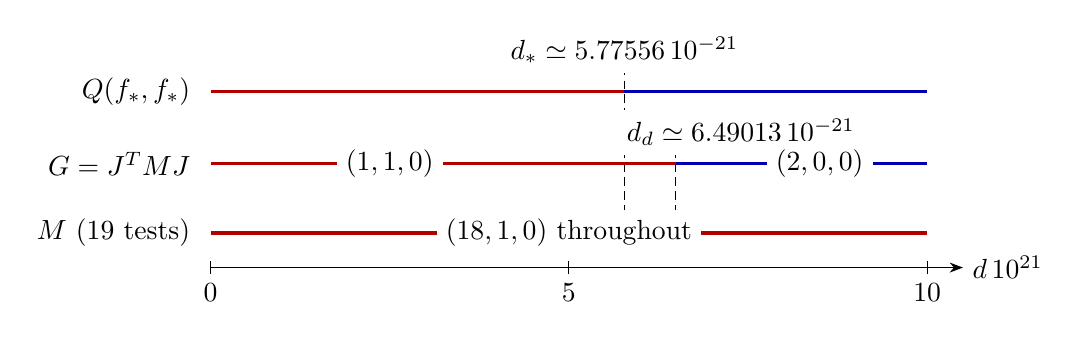
\begin{tikzpicture}[x=0.91cm,y=0.8cm,>=Stealth]
\draw[->] (0,0)--(10.5,0) node[right] {$d\,10^{21}$};
\foreach \x in {0,5,10} {\draw(\x,.10)--(\x,-.10) node[below] {$\x$};}
\draw[densely dashed] (5.77556,.2)--(5.77556,3.15);
\draw[densely dashed] (6.49013,.2)--(6.49013,2.25);
\node[anchor=east] at (-.15,2.8) {$Q(f_*,f_*)$};
\draw[very thick,red!70!black] (0,2.8)--(5.77556,2.8);
\draw[very thick,blue!70!black] (5.77556,2.8)--(10,2.8);
\node[fill=white] at (5.77556,3.45) {$d_*\simeq5.77556\,10^{-21}$};
\node[anchor=east] at (-.15,1.65) {$G=J^TMJ$};
\draw[very thick,red!70!black] (0,1.65)--(6.49013,1.65);
\draw[very thick,blue!70!black] (6.49013,1.65)--(10,1.65);
\node[fill=white] at (7.4,2.15) {$d_d\simeq6.49013\,10^{-21}$};
\node[anchor=east] at (-.15,.55) {$M\ (19\text{ tests})$};
\draw[very thick,red!70!black] (0,.55)--(10,.55);
\node[fill=white] at (2.5,1.65) {$(1,1,0)$};
\node[fill=white] at (8.5,1.65) {$(2,0,0)$};
\node[fill=white] at (5,.55) {$(18,1,0)$ throughout};
\end{tikzpicture}
\caption{The original time is $t=-2+d$. Positions are displayed
to six digits; NF5 and NC12 retain the exact brackets. Red means
a negative direction is present; blue means this displayed
restriction is positive. The complete nineteen-test form stays
nondegenerate and indefinite across both crossings, by NF8--19.
Rodgers--Tao's original theta data enter through WR1--5.}
\end{figure}

\clearpage
\section{The original two-test connection at the certified determinant zero}
\label{sec:schur-connection-support}

\paragraph{SC1. Original objects and the certified point.}
We keep the original Rodgers--Tao heat family and clock:
\[
 H_t(Z)=\int_0^\infty e^{tu^2}\Phi(u)\cos(Zu)\,du,\qquad
 \partial_tH_t=-\partial_Z^2H_t,\qquad
 H_0(Z)=\frac18\xi_R\!\left(\frac12+\frac{iZ}{2}\right).
 \tag{SC1}
\]
The author source is Brad Rodgers and Terence Tao,
\href{https://arxiv.org/abs/1801.05914v5}{\emph{The de Bruijn--Newman
constant is non-negative}}, version 5, author equations
\texttt{phidef}, \texttt{htdef}, \texttt{hoz}, and \texttt{sas}.
The retained original TeX has canonical source ID
\texttt{RODGERS-TAO-ARXIV-1801.05914-v5}.
Only those defining passages are used here. The complete-root
receiving proof is WR1--5; the fixed tests and support carrier are
NC1--2 and NC21, retained with this component. In particular,
\[
 \begin{gathered}
 f_*(Z)=\sum_{i=0}^{18}c_iZ^{-2i-1},\quad
 c_i=1000^i n_i/10^{120},\quad g_0(Z)=Z^{-1},\\
 Q=\sum_{i,j=0}^{18}c_ic_jS_{i+j+1},\qquad
 B=\sum_{i=0}^{18}c_iS_{i+1},\qquad A=S_1=M_1/M_0>0 .
 \end{gathered}\tag{SC2}
\]
The integers \(n_i\) are the unrounded supplied vector, retained in
\texttt{rational\_witness.json} with SHA256
\path{85314e9fb3115647b7f03a5e00f1b5512c4b23c9280a753f3cf2cababdfed4ac}.
All traces here receive the entire original zero divisor. We use
the ordered original basis \((f_*,g_0)\) of \(V\); its independence
also follows from \(c_{18}=10^{54}\ne0\).

Write
\[
 G(t)=\begin{pmatrix}Q&B\\B&A\end{pmatrix},\quad
 \Delta(t)=\det G=QA-B^2,\quad
 \beta=B/A,\quad S=Q-B^2/A,\quad \Delta=AS.
 \tag{SC3}
\]
The certified calculation in
\path{CERTIFIED_SCHUR_TRANSITION.json} and
\path{certify_schur_transition.py} proves that \(\Delta\) has
one simple zero \(t_d=-2+d_d\) on \([-2,-2+10^{-20}]\), with
\[
 \frac{862686317576371313926327932467260436}{2^{120}10^{20}}
 <d_d<
 \frac{862686317576371313926327932467260437}{2^{120}10^{20}}.
 \tag{SC4}
\]
The proof uses the complete theta interval bounds from the
companion calculation: \(\Delta''>0\) on the interval,
\(\Delta'(-2)>0\), strict opposite endpoint signs, and 120
rational bisections with strict signs. This component receives
that established point; it does not repeat the quadrature.
The same receipt proves \(A_d>0\), \(B_d>0\), and
\[
 \begin{split}
 7.34673724543500384324\,10^{-26}
 &<s_1:=S'(t_d)=\Delta'(t_d)/A_d
 <7.34673724543500384326\,10^{-26},\\
 7.51503947413203068735\,10^{-23}
 &<\beta_d<7.51503947413203068736\,10^{-23}.
 \end{split}\tag{SC5}
\]
These bounds are outward enlargements of the retained exact binary
endpoints. Subscripts \(d\) below denote evaluation at this point.

The local coordinate is the explicit translation
\(\zeta=t-t_d\), so \(d\zeta=dt\); the physical time and the
arithmetic coordinate \(s=\frac12+iZ/2\) are unchanged.
NC1--4 give real analytic entries and their holomorphic extensions
near \(t_d\). Shrink a complex disk so that \(A\ne0\) throughout
and \(S\) has only its simple zero at \(\zeta=0\).
For complex \(\zeta\) we use the holomorphic symmetric bilinear
extension \(v^TGw\). On the real interval, \(G\) is real symmetric
and defines the original Hermitian form \(v^*Gw\). These two uses
of transpose and conjugate transpose will be kept explicit.

\paragraph{SC2. The exact Schur morphism, including its derivative.}
Define
\[
 P=\begin{pmatrix}1&0\\-\beta&1\end{pmatrix},\qquad
 D=\begin{pmatrix}S&0\\0&A\end{pmatrix},\qquad
 C=P^{-1}P'=\begin{pmatrix}0&0\\-\beta'&0\end{pmatrix}.
 \tag{SC6}
\]
Direct multiplication gives \(P^TGP=D\) and \(\det P=1\).
Thus \(P\) is a holomorphic isometry from the Schur presentation
\((\mathbb C^2,D)\) to the original presentation
\((V,G)\), including the degenerate central fibre. The first
Schur basis vector maps to \(f_*-\beta g_0\); the second maps to
\(g_0\). No scalar factor has been removed from the metric.

On the punctured disk, set
\[
 \Omega=\Gamma\,dt,\qquad
 \Gamma=\frac12G^{-1}G'
 =\frac1{2AS}
 \begin{pmatrix}
 A Q'-B B'&A B'-B A'\\
 Q B'-B Q'&Q A'-B B'
 \end{pmatrix}.
 \tag{SC7}
\]
The horizontal equation is \(X'=-\Gamma X\).
Because \(G^T=G\) and \((G')^T=G'\),
\[
 G'=\Gamma^TG+G\Gamma.
 \tag{SC8}
\]
For horizontal column solutions \(x,y\), differentiating
\(x^TGy\) therefore gives zero. For real time and arbitrary complex
column solutions the same argument, with \(\Gamma^*=\Gamma^T\),
proves preservation of \(x^*Gy\). The connection is flat on the
punctured complex disk: both \(d\Omega\) and
\(\Omega\wedge\Omega\) vanish, since every factor is a multiple
of \(dt\).

For the change of variables \(x=Py\), the full transformed
coefficient is
\[
 \begin{split}
 \widetilde\Gamma
 &=P^{-1}\Gamma P+P^{-1}P'\\
 &=\frac12D^{-1}D'+\frac12(C-D^{-1}C^TD)\\
 &=\begin{pmatrix}
       S'/(2S)&A\beta'/(2S)\\
       -\beta'/2&A'/(2A)
    \end{pmatrix}.
 \end{split}\tag{SC9}
\]
To prove the middle equality, differentiate \(D=P^TGP\):
\[
 P^TG'P=D'-C^TD-DC,\qquad
 P^{-1}G^{-1}G'P=D^{-1}(D'-C^TD-DC).
\]
Add \(C\) after division by two. The correction
\(K=(C-D^{-1}C^TD)/2\) satisfies \(K^TD+DK=0\).
Consequently both displayed terms contribute to the same exact
compatibility equation \(D'=\widetilde\Gamma^TD+
D\widetilde\Gamma\). Deleting \(K\) changes the connection; it
is not the gauge transformation of SC7 unless \(\beta'=0\).

\paragraph{SC3. The residue in the original basis.}
Put
\[
 r=\binom{1}{-\beta_d},\qquad
 \ell=\binom{\beta_d}{1},\qquad
 G_d=A_d\ell\ell^T,\qquad
 \operatorname{adj}G_d=A_drr^T .
 \tag{SC10}
\]
The determinant derivative is \(\Delta'_d=A_ds_1\).
Dividing the adjugate formula for \(G^{-1}\) by its simple
determinant zero gives
\[
 R:=\operatorname{Res}_{t=t_d}\Omega
   =\frac{r r^TG'_d}{2s_1}.
 \tag{SC11}
\]
One also has \(r^TG'_dr=s_1\). Indeed
\((1,-\beta)G(1,-\beta)^T=S\), and the two differentiated-vector
terms vanish at \(t_d\), because \(G_dr=0\). It follows that
\[
 R^2=\tfrac12R,\quad
 \operatorname{tr}R=\tfrac12,\quad
 \operatorname{im}R=\mathbb Cr=\ker G_d,\quad
 \ker R=\ker(r^TG'_d).
 \tag{SC12}
\]
Every assertion follows directly from SC11 and
\(r^TG'_dr=s_1\ne0\): \(R\) has rank one, \(Rr=r/2\),
and its defining covector is nonzero.

For an explicit second line, set
\[
 a=\frac{A_d\beta'_d}{s_1},\qquad
 v=\binom{-a}{1+\beta_da},\qquad
 T=(r\ \ v)=
 \begin{pmatrix}1&-a\\-\beta_d&1+\beta_da\end{pmatrix}.
 \tag{SC13}
\]
The identity
\[
 \frac{r^TG'_d}{s_1}=(1+\beta_da,\ a)
 \tag{SC14}
\]
follows by differentiating \(B=A\beta\) and
\(Q=S+A\beta^2\). Hence \(Rv=0\), \(\det T=1\), and
\[
 T^{-1}RT=\Lambda=\begin{pmatrix}1/2&0\\0&0\end{pmatrix},
 \qquad v^TG_dv=A_d.
 \tag{SC15}
\]
In the Schur presentation,
\[
 \widetilde R=
 \begin{pmatrix}1/2&a/2\\0&0\end{pmatrix},\qquad
 R=P_d\widetilde RP_d^{-1}
 =\frac12\begin{pmatrix}
 1+\beta_da&a\\-\beta_d(1+\beta_da)&-\beta_da
 \end{pmatrix}.
 \tag{SC16}
\]
The derivative \(P^{-1}P'\) is analytic, so it contributes no
residue, even though it is essential to the full connection.
For the actual input, the certified residue is enclosed by
\[
\begin{aligned}
 R_{11}&\in(0.56568826983857144053,\,0.56568826983857144055),\\
 R_{12}&\in(8.74090815686078356647,\,8.74090815686078356648)10^{20},\\
 R_{21}&\in(-4.25116967789031619450,\,-4.25116967789031619449)10^{-23},\\
 R_{22}&\in(-0.06568826983857144054,\,-0.06568826983857144053).
\end{aligned}
 \tag{SC17}
\]
The exact rank, trace, eigenvalues, and lines are SC11--16;
independent rounding of matrix entries is not used to prove them.

\paragraph{SC4. A convergent gauge retaining every analytic coefficient.}
SC7 and the simple zero imply
\(\Gamma=R/\zeta+J(\zeta)\), with \(J\) holomorphic at zero.
Write \(J=\sum_{j\ge0}J_j\zeta^j\).
There is a unique holomorphic matrix \(F\), with \(F(0)=I\),
satisfying
\[
 F^{-1}\Gamma F+F^{-1}F'=\frac R\zeta .
 \tag{SC18}
\]
Here and below the disk may be made smaller without altering the
physical parameter or the matrix entries.

We prove existence, convergence, and invertibility. Substitution
of \(F=\sum_{k\ge0}F_k\zeta^k\), \(F_0=I\), into
\(\zeta F'=FR-RF-\zeta JF\) gives the exact recurrence
\[
 (kI+\operatorname{ad}_R)F_k
   =-\sum_{j=0}^{k-1}J_jF_{k-1-j},\qquad k\ge1,
 \quad \operatorname{ad}_R(U)=RU-UR .
 \tag{SC19}
\]
In the \(T\) basis, each entry on the left is multiplied by
\(k+\lambda_i-\lambda_j\), where
\((\lambda_1,\lambda_2)=(1/2,0)\). The four multipliers are
\(k,k+1/2,k-1/2,k\), none zero. This proves formal existence
and uniqueness.

For convergence use
\(\|U\|_*=\|T^{-1}UT\|_1\), where \(\|\cdot\|_1\) is the
induced column-sum matrix norm. This norm is submultiplicative,
and \(\|I\|_*=1\). Entrywise division by the four multipliers
shows
\[
 \|(kI+\operatorname{ad}_R)^{-1}U\|_*
 \le\frac{\|U\|_*}{k-1/2}\le\frac2k\|U\|_*.
 \tag{SC20}
\]
Choose \(\rho>0\) such that \(J\) is holomorphic on a neighborhood
of the closed disk of radius \(\rho\), and let
\(M=\max_{|\zeta|=\rho}\|J(\zeta)\|_*\).
Cauchy's coefficient formula gives
\(\|J_j\|_*\le M\rho^{-j}\). Therefore
\[
 \|F_k\|_*\le\frac2k\sum_{j=0}^{k-1}
 M\rho^{-j}\|F_{k-1-j}\|_*.
\]
The nonnegative majorant coefficients \(g_k\) defined by equality
and \(g_0=1\) are the Taylor coefficients of
\[
 g(z)=\exp\!\left(2M\int_0^z\frac{dw}{1-w/\rho}\right)
     =(1-z/\rho)^{-2M\rho}.
 \tag{SC21}
\]
This function is analytic for \(|z|<\rho\), with nonnegative
Taylor coefficients, including the case \(M=0\).
Induction gives \(\|F_k\|_*\le g_k\); hence \(F\) converges
absolutely and locally uniformly there. Its differentiated
series satisfies SC18 wherever it is invertible, initially on
a disk because \(F(0)=I\). Taking the trace of that equation yields
\[
 (\det F)'=-(\operatorname{tr}J)\det F,\qquad
 \det F(\zeta)=
 \exp\!\left(-\int_0^\zeta\operatorname{tr}J(w)\,dw\right).
 \tag{SC22}
\]
The equality first holds on that smaller disk and then throughout
the disk by the identity theorem, since both sides are analytic.
Its right side never vanishes. Thus \(F\) is invertible wherever
the preceding convergence construction is used. All coefficients
of \(J\) enter SC19; no analytic remainder has been dropped.

\paragraph{SC5. An exact metric identity and the original real inertia.}
Set \(E=FT\). Then SC18 and SC15 give
\[
 E^{-1}\Gamma E+E^{-1}E'=\frac{\Lambda}{\zeta}.
 \tag{SC23}
\]
The following identity retains both original constants:
\[
 E(\zeta)^T G(t_d+\zeta)E(\zeta)
   =\begin{pmatrix}s_1\zeta&0\\0&A_d\end{pmatrix}.
 \tag{SC24}
\]
To prove it, denote the left side by \(K\).
It is holomorphic at zero. Differentiate using SC8 and SC23:
\(\zeta K'=\Lambda^TK+K\Lambda\).
If \(K_{ij}=\sum_{n\ge0}k_{ij,n}\zeta^n\), then
\[
 (n-\lambda_i-\lambda_j)k_{ij,n}=0.
\]
Thus \(K_{11}\) is a constant multiple of \(\zeta\),
\(K_{22}\) is constant, and \(K_{12}=K_{21}=0\), because
\(1/2\) is not a nonnegative integer. At zero,
\(E(0)=T\); hence \(K_{22}(0)=v^TG_dv=A_d\).
For the first entry, the differentiated-vector terms vanish
because \(G_dr=0\), giving \(K'_{11}(0)=r^TG'_dr=s_1\).
This proves SC24.

Reality of the input and SC19 shows that every \(F_k\) is real.
For real \(\zeta\), SC24 is therefore also an exact Hermitian
congruence, with \(E^*=E^T\). Since \(s_1,A_d>0\), the
original two-test form has one negative and one positive
eigenvalue for sufficiently small negative \(\zeta\), one
zero and one positive eigenvalue at \(\zeta=0\), and two
positive eigenvalues for sufficiently small positive \(\zeta\).
These are statements about the fixed subspace
\(\operatorname{span}_{\mathbb C}(f_*,g_0)\). No positivity
statement for the full nineteen-dimensional test space follows
from this two-dimensional congruence.

The complete morphism from the diagonal presentation in SC24
to the Schur presentation is \(Y=P^{-1}E\). Direct substitution
of SC9 and SC23 proves
\[
 Y^TDY=\operatorname{diag}(s_1\zeta,A_d),\qquad
 Y^{-1}\widetilde\Gamma Y+Y^{-1}Y'=\Lambda/\zeta.
 \tag{SC25}
\]
The composition \(PY=E\) holds on the whole disk, including zero
for the metrics and on the punctured disk for the connections.
This proves both changes of presentation and their exact
composition; it also exhibits where the derivative correction
in SC9 is received.

\paragraph{SC6. Full local monodromy and the based reflection.}
On the logarithmic covering of the punctured disk a horizontal
fundamental matrix is
\[
 X(\zeta)=F(\zeta)\exp(-R\log\zeta).
 \tag{SC26}
\]
Differentiation using SC18 verifies \(X'=-\Gamma X\);
both factors are invertible. A positive meridian adds \(2\pi i\)
to \(\log\zeta\). Since \(R^2=R/2\),
\[
 e^{-2\pi iR}=I-4R,\qquad (I-4R)^2=I.
 \tag{SC27}
\]
For example, expand the exponential on
\(\mathbb C^2=\operatorname{im}R\oplus\ker R\):
it is multiplication by \(e^{-\pi i}=-1\) on the first
line and by \(1\) on the second.

Fix a base point \(\zeta_b\ne0\) in the disk. Parallel transport
around a positive meridian, in the actual original basis at
that point, is
\[
 \mathcal M_b
 =F_b(I-4R)F_b^{-1},\quad
 \operatorname{im}(\mathcal M_b-I)=F_b\mathbb Cr,\quad
 \ker(\mathcal M_b-I)=F_b\mathbb Cv.
 \tag{SC28}
\]
Indeed analytic continuation of SC26 is right multiplication by
\(I-4R\), so the based transport is \(X_b(I-4R)X_b^{-1}\).
The exponential in \(X_b\) commutes with \(R\), yielding SC28.
Thus the original-basis matrix at a nonzero base point involves
the full convergent \(F_b\). Its two invariant lines tend to
\(\mathbb Cr\) and \(\mathbb Cv\) as the base point tends to zero.
Changing the base point by parallel transport conjugates the
matrix, as follows directly from the same fundamental solution.

There is also an exact formula using the original metric.
Put \(u_b=F_br\), \(w_b=F_bv\), and \(G_b=G(t_d+\zeta_b)\).
SC24 gives
\[
 u_b^TG_bu_b=s_1\zeta_b,\qquad
 w_b^TG_bw_b=A_d,\qquad u_b^TG_bw_b=0.
\]
Consequently
\[
 \mathcal M_b
   =I-\frac{2u_bu_b^TG_b}{s_1\zeta_b},\qquad
 \mathcal M_b^TG_b\mathcal M_b=G_b,\qquad
 \det\mathcal M_b=-1 .
 \tag{SC29}
\]
To verify the first equality, apply its right side to the
basis \((u_b,w_b)\): it sends the first vector to its negative
and fixes the second, exactly as SC28. The other identities
follow either by the same basis calculation or by SC8.
For real base points \(u_b,w_b,\mathcal M_b\) are real, so the
orthogonality identity also uses conjugate transpose for the
original Hermitian form.

The fundamental group of the punctured disk is generated by
one meridian, and a loop of winding number \(k\) has holonomy
\(\mathcal M_b^k\); its determinant is \((-1)^k\).
Alternatively \(\operatorname{tr}\Gamma=
\frac12(\log\Delta)'\), and the determinant equation for
horizontal transport gives the same character, since \(\Delta\)
has a simple zero. This also verifies the sign in the
horizontal convention of SC7.

\paragraph{SC7. Supported determinant, radical, and exact quotient.}
Let \(L\) be the original bounded distributive lattice. For a
complex vector space \(W\), retain the full carrier
\[
 M_L(W)=(W\times\{1_L\})\cup(\{0\}\times L).
 \tag{SC30}
\]
Addition is \((w,\lambda)+(z,\mu)=(w+z,\lambda\vee\mu)\);
scalar multiplication by \((c,\nu)\in M_L(\mathbb C)\) is
\((cw,\nu\wedge\lambda)\). The zero is
\(\tau=(0,0_L)\), and \(e=(0,1_L)\) is the top supported
zero. Here \(\tau\) denotes this zero element, and the local
time displacement remains \(\zeta\).
The operations stay in the stated carrier: any amplitude
different from zero forces every required support to be top.
Associativity and the distributive laws follow from those of
vector addition, scalar multiplication, and the distributivity
of \(L\). Complex conjugation acts on the amplitude and fixes
the support.

For real \(t\), the complete sesquilinear lift of the form is
\[
 \widehat Q_t((z,\lambda),(w,\mu))
  =(z^*G(t)w,\lambda\wedge\mu).
 \tag{SC31}
\]
Additivity uses
\((\lambda\vee\nu)\wedge\mu
=(\lambda\wedge\mu)\vee(\nu\wedge\mu)\);
scalar compatibility uses associativity of meet and the
original sesquilinearity. Thus SC31 proves the lift, with the
amplitude projection commuting with the original form.
For complex time the same formula with \(z^T\) supplies the
holomorphic bilinear version.

The entries of the original Gram array have top support.
Taking its determinant in that top fibre gives
\[
 \widehat\Delta(t)
 =(Q,1_L)(A,1_L)+(-1,1_L)(B,1_L)^2
 =(\Delta(t),1_L).
 \tag{SC32}
\]
Hence \(\widehat\Delta(t_d)=e\). If \(0_L\ne1_L\), this is
distinct from \(\tau\); if \(L\) has one element the labels
coincide, exactly as the definition requires. In every case the
amplitude determinant is zero and has no multiplicative
inverse. The supported label does not supply an inverse for
the matrix in SC7 at \(t_d\).

At the central fibre, the exact sequence of ordinary vector
spaces is
\[
 0\longrightarrow\mathbb Cr
 \ \xrightarrow{\ \iota\ }\ V
 \ \xrightarrow{\ \ell^T\ }\ \mathbb C
 \longrightarrow0,\qquad
 G_dz=A_d\ell\,(\ell^Tz).
 \tag{SC33}
\]
Here coordinates in \(V\) refer to the original ordered tests,
and \(G_d\) maps to the coordinate dual space. The map
\(\ell^T\) is surjective, since \(\ell^T(0,1)^T=1\);
its kernel is exactly \(\mathbb Cr\). SC10 proves the
factorization. Thus the image of the Gram map is
\(\mathbb C\ell\), the radical is \(\mathbb Cr\), and the
quotient \(V/\mathbb Cr\) receives the nondegenerate form
\[
 Q_d(z,w)=A_d\,\overline{\ell^Tz}\,(\ell^Tw).
 \tag{SC34}
\]
This is the full quotient form, including \(A_d\).

Every linear map \(U:W\to W'\) has the explicit supported lift
\(\widehat U(w,\lambda)=(Uw,\lambda)\).
It preserves addition and supported scalar multiplication by
the displayed formulas. Composition and amplitude projection
commute with this lift. Therefore SC33, the maps \(P,E,Y\),
and all their inverses where present have exact supported
receivers without losing any zero label.
For the degenerate Gram map the amplitude radical carrier is
\[
 \mathcal N_L=(\mathbb Cr\times\{1_L\})
               \cup(\{0\}\times L).
 \tag{SC35}
\]
The inverse image of the full zero-amplitude carrier under
\(\widehat G_d\) is exactly \(\mathcal N_L\): this follows
from \(\ker G_d=\mathbb Cr\), with each support retained.
For \(c\ne0\), \(\widehat G_d(cr,1_L)=(0,1_L)\), and its
pairing with every top-supported vector is \(e\).
For an argument supported at \(\lambda\), the output support
is the stated meet, including when its amplitude vanishes.
This gives the precise relation between the amplitude radical
and the retained supported zeros. In particular it does not
replace all zero amplitudes by the additive zero \(\tau\).

At each nonzero base point the invertible holonomy
\(\mathcal M_b\) lifts to
\(\widehat{\mathcal M}_b(z,\lambda)=(\mathcal M_bz,\lambda)\).
It preserves SC31 for real base points, because of SC29, and
fixes every labelled zero \((0,\lambda)\). On amplitudes it
reverses \(F_b\mathbb Cr\) and fixes \(F_b\mathbb Cv\).
Its supported determinant is \((-1,1_L)\).

\paragraph{SC8. What the local holonomy receives.}
Equations SC18--29 calculate the complete local connection of
the actual two-test form at the established \(t_d\).
They prove that its local holonomy receives a simple loss of
rank in that fixed Gram space: the residue image is the
central radical, and the nonzero-fibre negative eigenspace of
the holonomy converges to it. The analytic transport of that
line is given by the convergent \(F\), whose coefficients are
SC19, and its exact metric value is \(s_1\zeta\).

The connection is connected to the original heat family by the
explicit complete-root trace map SC2 and its original-clock
derivatives NC3. Its singularity is the zero of the determinant
of those received pairings. This calculation neither
identifies that determinant with \(H_t\) nor asserts a zero of
\(H_t\) at a specified spatial point. The certified physical
time is the strictly negative number in SC4, and remains near
\(-2\) after every displayed change of frame. Thus the local
reflection is established at that two-test transition; no
claim of an RH proof, disproof, or endpoint transition at
\(t=0\) is made.

\paragraph{SC9. Reproducible finite verification.}
The companion \texttt{check\_schur\_connection.py} uses exact
rational operations. It checks SC6--16 on explicit polynomial
analytic metrics with nonconstant \(A,S/\zeta,\beta\); computes
the first eight convergent-gauge coefficients using SC19;
checks the differential equation and SC24 to those orders;
and verifies the reflection identities. These finite checks
test signs, transpose order, noncommuting products, and the
frame derivative correction. SC18--24 supply the separate
all-orders convergence proof. The checker also reads the exact
binary endpoints of the actual receipt to verify every
outward enlargement displayed in SC4--5 and SC17, without
repeating any numerical integration.

\paragraph{SC10. The original nineteen-test inclusion and its full connection.}
The companion complete-theta calculation proves that the
original nineteen-test matrix is nondegenerate throughout
\(I=[-2,-2+10^{-20}]\), with inertia \((18,1,0)\) in the order
(positive, negative, zero). The exact receiver here is
\[
 \begin{gathered}
 \mathcal V=\operatorname{span}_{\mathbb C}
      \{h_i(Z)=Z^{-2i-1}:0\le i\le18\},\qquad
 \mathcal K(t)=(S_{i+j+1}(t))_{0\le i,j\le18},\\
 D_0=\operatorname{diag}(1000^i)_{i=0}^{18},\qquad
 M=D_0\mathcal KD_0,\qquad w_i=n_i/10^{120},\\
 J_Z=(c,e_0),\qquad
 J=D_0^{-1}J_Z=(w,e_0)
 :\mathbb C^2\longrightarrow\mathbb C^{19},\qquad
 J^TMJ=G .
 \end{gathered}\tag{SC36}
\]
These are both original coefficient presentations. The
unscaled coordinate map sends \(z\) to \(\sum z_i h_i\).
The NF1 coordinate map sends \(x\) to
\(\sum x_i1000^i h_i\); the exact morphism between the
coordinates is \(z=D_0x\). Thus \(J_Z\) and \(J\) both give
the original constant inclusion of \((f_*,g_0)\), with no
alteration of spatial variable, heat clock, or rational test.
Since \(w_{18}=1\), \(J\) is injective. We use the NF1
symbols \(M,J\) below. The supplied proof receipt is
\texttt{UNIFORM\_FULL\_FLAG\_RECEIPT.json}: it encloses the
lower eighteen-dimensional fixed-frame perturbation norm
below \(1/20\), and the attained final Schur complement in
\[
 (-2.403366914664958469,\,-2.364761442970871715)\,10^{-46}.
 \tag{SC37}
\]
The companion argument retains all theta, Taylor, and
fifth-derivative remainder bounds. We use its established
nondegeneracy at the actual \(t_d\); these eighteen positive
directions and one negative direction therefore coexist with
the two-test transition proved above.

Because \(\det M(t_d)\ne0\), it remains nonzero on a complex
disk about \(t_d\). The full original-basis connection is
\[
 \Gamma_{\rm full}=\tfrac12M^{-1}M',\qquad
 M'=\Gamma_{\rm full}^TM+M\Gamma_{\rm full}.
 \tag{SC38}
\]
It is holomorphic throughout this disk. Its horizontal
fundamental matrix \(U\), with \(U(0)=I_{19}\), is holomorphic
and invertible there after shrinking the disk. For completeness,
if \(\Gamma_{\rm full}=\sum_{j\ge0}L_j\zeta^j\), its
coefficients are uniquely given by
\[
 nU_n=-\sum_{j=0}^{n-1}L_jU_{n-1-j},\qquad U_0=I_{19}.
 \tag{SC39}
\]
For a submultiplicative matrix norm, Cauchy bounds
\(\|L_j\|\le C\rho^{-j}\) give the convergent majorant
\((1-z/\rho)^{-C\rho}\), by the same coefficient comparison
as SC20--21, now with factor \(1/n\). Thus the series converges.
The determinant satisfies
\((\det U)'=-\operatorname{tr}(\Gamma_{\rm full})\det U\)
and is the exponential of a holomorphic integral. Hence it
does not vanish. This proves that full parallel transport is
\(U(t_2)U(t_1)^{-1}\) and has identity holonomy around every
loop in this disk, including a loop surrounding \(t_d\).
For the unscaled Laurent coordinates the coefficient is
\(\Gamma_{\mathcal K}=\mathcal K^{-1}\mathcal K'/2\).
Since \(D_0\) is constant, differentiation and inversion give
the exact gauge identity
\(\Gamma_{\rm full}=D_0^{-1}\Gamma_{\mathcal K}D_0\).
Thus \(D_0\) intertwines their horizontal equations and
parallel transports, including the identity local holonomy.

\paragraph{SC11. Exact compression and the complementary term.}
On the punctured disk define
\[
 \begin{split}
 J^\dagger&=G^{-1}J^TM:\mathbb C^{19}\longrightarrow\mathbb C^2,\\
 \Pi&=JJ^\dagger:\mathbb C^{19}\longrightarrow\mathbb C^{19},\\
 W&=(I_{19}-\Pi)\Gamma_{\rm full}J .
 \end{split}\tag{SC40}
\]
The dagger denotes this metric adjoint and left inverse; it
is the stated meromorphic holomorphic formula, not a
conjugation of complex time. On real time it is also the
adjoint of the original Hermitian metrics, since \(J\) is
real. From SC36,
\[
 \begin{gathered}
 J^\dagger J=I_2,\qquad \Pi^2=\Pi,\qquad
 \Pi^TM=M\Pi,\\
 \operatorname{im}\Pi=\operatorname{im}J,\qquad
 \ker\Pi=\ker(J^TM)=(\operatorname{im}J)^{\perp_M}.
 \end{gathered}\tag{SC41}
\]
Indeed \(J^\dagger J=G^{-1}G\); idempotence and the image
follow immediately. Since \(G^{-1}\) is symmetric,
\(M\Pi=MJG^{-1}J^TM\) is symmetric. Finally \(J\) is
injective and \(G^{-1}\) invertible, proving the kernel
identity.
In the unscaled presentation define
\(J_Z^\dagger=G^{-1}J_Z^T\mathcal K\) and
\(\Pi_Z=J_ZJ_Z^\dagger\). SC36 gives
\[
 J^\dagger=J_Z^\dagger D_0,\qquad
 \Pi=D_0^{-1}\Pi_ZD_0 .
\]
Thus the projection, its image, kernel, and residue below
are carried to the unscaled original Laurent coordinates
by the same exact constant isomorphism \(D_0\).

Differentiating SC36 uses \(J'=0\). Since
\(M\Gamma_{\rm full}=M'/2\), it gives the exact
compression and decomposition
\[
 \begin{split}
 J^\dagger\Gamma_{\rm full}J
   &=\tfrac12G^{-1}J^TM'J=\tfrac12G^{-1}G'=\Gamma,\\
 \Gamma_{\rm full}J&=J\Gamma+W,\qquad
 J^TMW=0 .
 \end{split}\tag{SC42}
\]
Thus the compressed connection is the orthogonally projected
full connection on this fixed subspace for every nonzero
\(\zeta\). Its unprojected complementary term is the displayed
\(W\); it is not removed from the full equation. For a
compressed horizontal solution \(y'=-\Gamma y\), the
original ambient vector \(x=Jy\) obeys
\[
 x'+\Gamma_{\rm full}x=W y.
 \tag{SC43}
\]
This follows by substitution in SC42. It states precisely
which ambient covariant derivative remains when one uses
compressed horizontal transport.

\paragraph{SC12. Nilpotent projection residue and cancellation.}
Let \(n=Jr\ne0\). From SC10--11 one has the Laurent expansions
\[
 \begin{split}
 G^{-1}&=\frac{rr^T}{s_1\zeta}+\hbox{a holomorphic matrix},\\
 \operatorname{Res}J^\dagger&=\frac{r n^TM_d}{s_1},\\
 K_\Pi:=\operatorname{Res}\Pi&=\frac{n n^TM_d}{s_1}.
 \end{split}\tag{SC44}
\]
In particular
\[
 K_\Pi\ne0,\qquad K_\Pi^2=0,\qquad
 \operatorname{im}K_\Pi=\mathbb Cn,\qquad
 \ker K_\Pi=\ker(n^TM_d).
 \tag{SC45}
\]
To prove these assertions, observe that
\(n^TM_dn=r^TG_dr=0\). Since \(M_d\) is invertible and
\(n\ne0\), the row \(n^TM_d\) is nonzero. The displayed
outer product therefore has rank one and square zero,
with the indicated image and kernel. This also proves that
the pole of \(\Pi\) is a genuine pole, while the ambient
connection remains holomorphic.

The singular parts in SC42 cancel exactly:
\[
 \operatorname{Res}(J\Gamma)=JR,\qquad
 \operatorname{Res}W=-JR,\qquad
 \operatorname{Res}(\Gamma_{\rm full}J)=0 .
 \tag{SC46}
\]
One proof is the exact analytic decomposition SC42.
An independent calculation gives
\[
 K_\Pi(\Gamma_{\rm full})_dJ
  =\frac{n n^TM_d(\Gamma_{\rm full})_dJ}{s_1}
  =\frac{Jr\,r^TJ^TM'_dJ}{2s_1}
  =JR ,
 \tag{SC47}
\]
which proves SC46 directly from the projection's principal
part. Since \(J\) is injective and \(R\ne0\), neither residue
being cancelled is zero.

At the central fibre the exact geometric relation is
\[
 \operatorname{im}J\cap(\operatorname{im}J)^{\perp_{M_d}}
     =\mathbb Cn .
 \tag{SC48}
\]
Indeed \(Jz\) belongs to the intersection exactly when
\(J^TM_dJz=G_dz=0\); SC12 identifies those \(z\) as
\(\mathbb Cr\). The two spaces have dimensions \(2\) and
\(17\), because \(J^TM_d\) has rank two. They have
one-dimensional intersection at \(t_d\), so their sum there
has dimension \(18\). For \(\zeta\ne0\), SC41 gives instead
their direct sum as the full nineteen-dimensional space.
The line \(\mathbb Cn\) is isotropic in the nondegenerate
ambient metric, but is not an ambient radical: \(M_dn\ne0\).
This follows from invertibility, with its exact nonzero
covector already displayed in SC44.
In fact the limiting sum has the precise identification
\[
 \operatorname{im}J+(\operatorname{im}J)^{\perp_{M_d}}
   =\ker(n^TM_d)=\ker K_\Pi .
 \tag{SC49}
\]
For \(Jz\), the row \(n^TM_d\) gives
\(r^TG_dz=0\). It also vanishes on the orthogonal complement
because \(n\in\operatorname{im}J\). Thus the sum lies in that
kernel. Both have dimension eighteen, the latter because
\(n^TM_d\ne0\), proving equality.
Consequently the projection residue induces the exact
isomorphism
\[
 \mathbb C^{19}/\bigl(\operatorname{im}J+
            (\operatorname{im}J)^{\perp_{M_d}}\bigr)
 \longrightarrow\mathbb Cn,\qquad
 [z]\longmapsto \frac{n(n^TM_dz)}{s_1}.
\]
It is well defined and injective by SC49, and surjective
by the image assertion in SC45. This identifies the
one-dimensional quotient determined by the failed
orthogonal direct sum with the central compressed radical.

The projection pole, its nilpotent residue, and the
complementary residue in SC46 are thus the exact maps
connecting the compressed reflection SC28 to the ambient
identity holonomy SC39. The full horizontal equation and
the compressed equation are related by SC43, with a
nonzero complementary meromorphic operator. Removing it
would replace the ambient equation. Every map in SC36 and
SC40--48 has its support-preserving lift as in SC30--35
where its matrix is defined. In particular \(J\) and \(M_d\)
remain defined and injective at the central fibre;
\(\widehat M_d(n,1_L)\) has nonzero amplitude, while its
compression by \(\widehat{J^T}\) has amplitude zero and
top support. This proves the relation of the retained
compressed zero to the nondegenerate original full form.

There is a direct identity between the two parallel transports.
Along any piecewise smooth path in the punctured disk starting
at \(b\), let \(\mathcal P_V(z,b)\) denote the compressed
transport, continued along that path, and put
\(\mathcal P_{\rm full}(z,w)=U(z)U(w)^{-1}\).
The full matrix \(U\) is single valued on the entire disk.
Variation of constants applied to SC43 gives
\[
 \begin{split}
 J\mathcal P_V(z,b)
   ={}&\mathcal P_{\rm full}(z,b)J\\
    &+\int_b^z
      \mathcal P_{\rm full}(z,w)\,
      W(w)\mathcal P_V(w,b)\,dw .
 \end{split}\tag{SC50}
\]
To prove the formula, differentiate
\(U(z)^{-1}J\mathcal P_V(z,b)\). The product rule and SC43
give \(U(z)^{-1}W(z)\mathcal P_V(z,b)\). Integrate on the
chosen path and multiply by \(U(z)\); its value at \(b\)
is \(U(b)^{-1}J\). For a positive meridian \(\gamma\) based
at \(b\), SC50 becomes
\[
 J(\mathcal M_b-I_2)
   =\int_\gamma U(b)U(w)^{-1}W(w)
          \mathcal P_V(w,b)\,dw
   =-4JF_bRF_b^{-1}\ne0 .
 \tag{SC51}
\]
The integrand uses its continued compressed solution along
the path; it is not asserted to be single valued on the
punctured disk. The final matrix is nonzero because \(J\)
is injective, \(F_b\) is invertible, and \(R\ne0\).
This identity identifies the entire difference of the two
holonomies through the retained complementary term.

\begin{figure}[p]
\centering
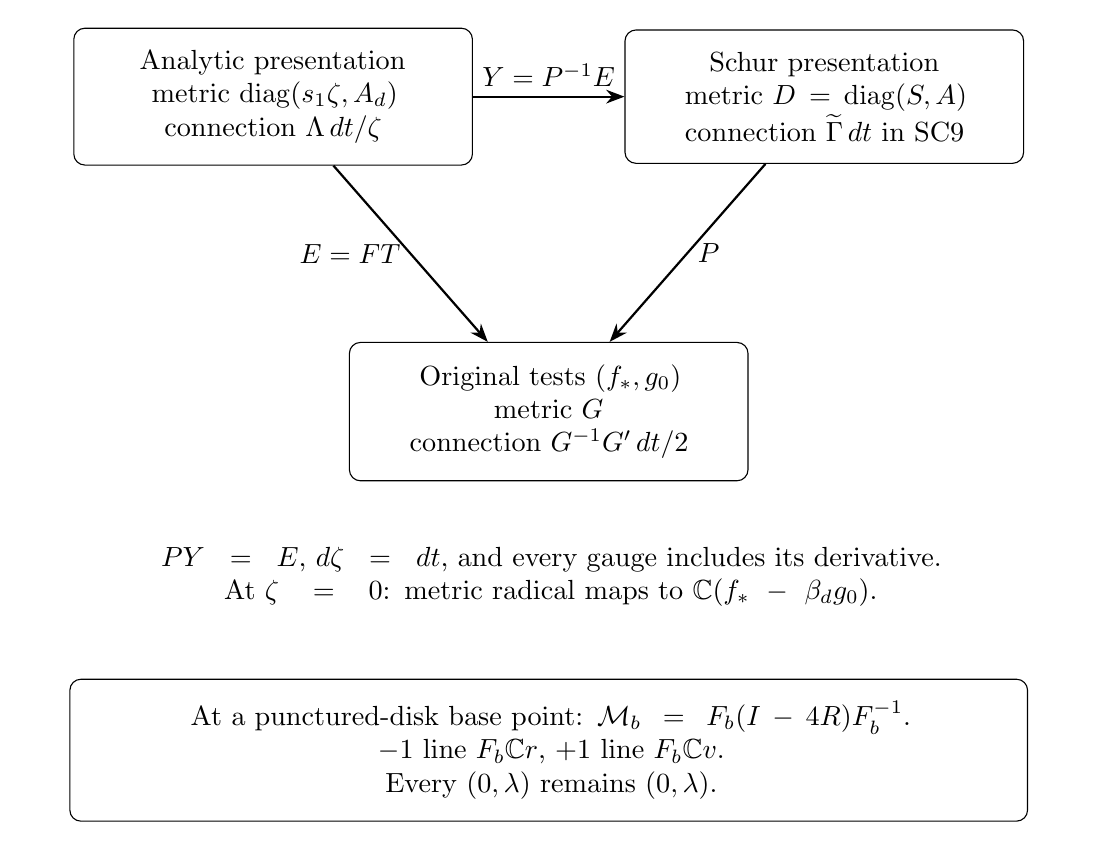
\begin{tikzpicture}[>=Stealth,
 box/.style={draw,rounded corners,align=center,text width=4.5cm,
 inner sep=8pt}]
\node[box] (diag) at (0,0)
 {Analytic presentation\\
 metric \(\operatorname{diag}(s_1\zeta,A_d)\)\\
 connection \(\Lambda\,dt/\zeta\)};
\node[box] (schur) at (7,0)
 {Schur presentation\\metric \(D=\operatorname{diag}(S,A)\)\\
 connection \(\widetilde\Gamma\,dt\) in SC9};
\node[box] (original) at (3.5,-4)
 {Original tests \((f_*,g_0)\)\\
 metric \(G\)\\ connection \(G^{-1}G'\,dt/2\)};
\draw[->,thick] (diag)--node[above]{\(Y=P^{-1}E\)} (schur);
\draw[->,thick] (diag)--node[left]{\(E=FT\)} (original);
\draw[->,thick] (schur)--node[right]{\(P\)} (original);
\node[align=center,text width=13cm] at (3.5,-6.1)
 {\(PY=E\), \(d\zeta=dt\), and every gauge includes its derivative.\\
 At \(\zeta=0\): metric radical maps to \(\mathbb C(f_*-\beta_dg_0)\).};
\node[box,text width=11.6cm] at (3.5,-8.3)
 {At a punctured-disk base point:
 \(\mathcal M_b=F_b(I-4R)F_b^{-1}\).\\
 \(-1\) line \(F_b\mathbb Cr\), \(+1\) line \(F_b\mathbb Cv\).\\
 Every \((0,\lambda)\) remains \((0,\lambda)\).};
\end{tikzpicture}
\caption{Exact maps of the original two-test metric and connection,
SC6--9 and SC18--35. The triangle commutes on the full disk for
metrics and on its punctured part for connections. The diagram
is a map diagram, not a spatial plot or a rescaled heat evolution.
The actual time is \(t=t_d+\zeta\), with \(t_d\) given in SC4.
The analytic source is Rodgers--Tao as cited in SC1; the original
test vector and its complete-trace receiver are NC1--2 and WR1--5.}
\label{fig:schur-connection-morphisms}
\end{figure}

\begin{figure}[p]
\centering
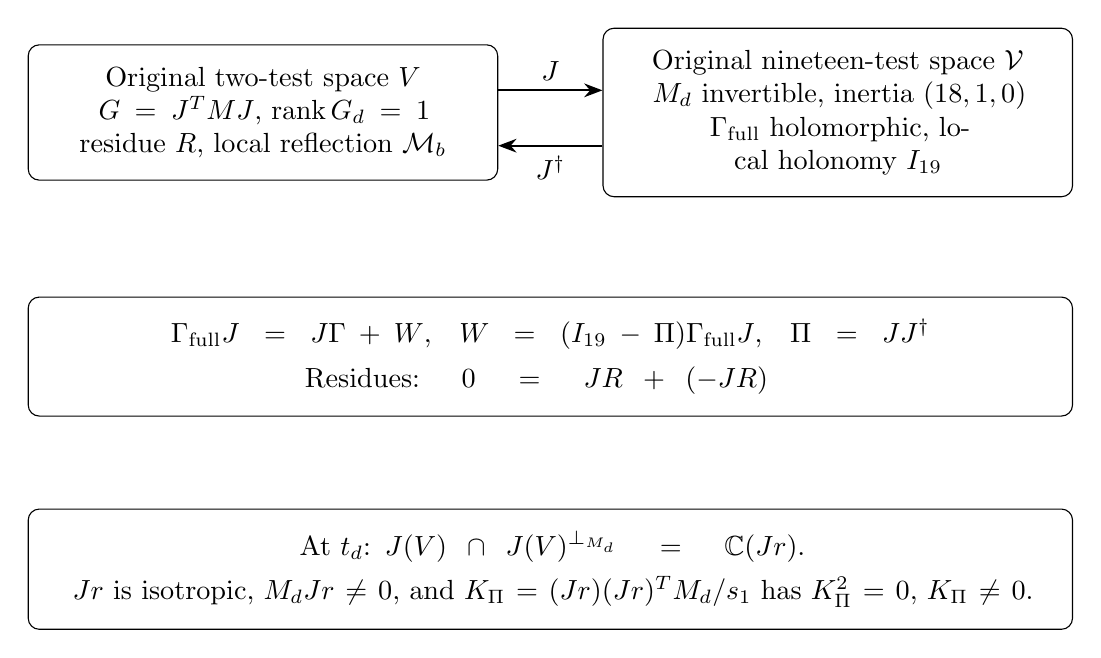
\begin{tikzpicture}[>=Stealth,
 box/.style={draw,rounded corners,align=center,text width=5.4cm,
 inner sep=8pt}]
\node[box] (small) at (0,0)
 {Original two-test space \(V\)\\
 \(G=J^TMJ\), \(\operatorname{rank}G_d=1\)\\
 residue \(R\), local reflection \(\mathcal M_b\)};
\node[box] (full) at (7.3,0)
 {Original nineteen-test space \(\mathcal V\)\\
 \(M_d\) invertible, inertia \((18,1,0)\)\\
 \(\Gamma_{\rm full}\) holomorphic, local holonomy \(I_{19}\)};
\draw[->,thick] ([yshift=8pt]small.east)
 --node[above]{\(J\)} ([yshift=8pt]full.west);
\draw[->,thick] ([yshift=-12pt]full.west)
 --node[below]{\(J^\dagger\)} ([yshift=-12pt]small.east);
\node[box,text width=12.7cm] (relation) at (3.65,-3.1)
 {\(\Gamma_{\rm full}J=J\Gamma+W\),\quad
 \(W=(I_{19}-\Pi)\Gamma_{\rm full}J\),\quad
 \(\Pi=JJ^\dagger\)\\[4pt]
 Residues: \(\quad 0=JR+(-JR)\quad\)};
\node[box,text width=12.7cm] at (3.65,-5.8)
 {At \(t_d\):
 \(J(V)\cap J(V)^{\perp_{M_d}}=\mathbb C(Jr)\).\\[4pt]
 \(Jr\) is isotropic, \(M_dJr\ne0\), and
 \(K_\Pi=(Jr)(Jr)^TM_d/s_1\) has
 \(K_\Pi^2=0\), \(K_\Pi\ne0\).};
\end{tikzpicture}
\caption{The exact relation between full and compressed transport,
SC36--48. The two arrows compose to \(I_2\) on the two-test
space and to \(\Pi\) on the full space away from \(t_d\).
The return arrow is meromorphic and its residue is given in
SC44. The complementary term \(W\) is retained; its pole
cancels the compressed pole. The original full theta receiver
is SC1--2 and NC1--4; the certified ambient nondegeneracy is
the complete-theta calculation in
\texttt{UNIFORM\_FULL\_FLAG\_RECEIPT.json}.}
\label{fig:ambient-compressed-cancellation}
\end{figure}

\clearpage
\section{The received rank passage and the original sixty-three-coordinate test}

The user supplied \emph{Boundary forcing, complete trace response,
and a finite-rank passage}, together with \texttt{witness63.json}.
The no-radical argument and the numerical claims below are credited
to that supplied continuation. We give their complete mathematical
receiving proof and independently reproduce the two supplied
sixty-three-coordinate values and sixty-four-dimensional inertias.
The other claimed rank-$32$/$33$ numerical cases are not asserted
as independently reproduced here. The original analytic source
remains Rodgers--Tao, cited in WR1 and NF2.

\paragraph{RPX1. The complete Laurent union has zero radical.}
Fix real physical time $b$ and put
$f_p(Z)=Z^{-1}p(Z^{-2})$, $p\in\mathbb C[X]$. For every nonzero
$p$ there is a $j\ge0$ such that
\[
 Q_b(f_p,Z^{-2j-1})=\sum_i\overline{p_i}S_{i+j+1}(b)\ne0.
 \tag{RPX1}
\]
Here $X$ denotes the rational function $Z^{-2}$; it is not a new
spatial coordinate. We prove the assertion. The original $H_b$ has
infinitely many distinct zeros. Indeed WR1 proves its order is at
most one and $H_b(0)>0$. Integration by parts on the real axis,
using integrability of the derivative of $e^{bu^2}\Phi(u)$, gives
$H_b(x)=O_b(1/|x|)$. If it had finitely many zeros, Hadamard's
factorization would make it a polynomial times $e^{a+cx}$.
Such a nonzero function cannot tend to zero at both real ends:
if $\Re c\ne0$ one end grows, while if $\Re c=0$ the modulus
is a nonzero polynomial modulus. Thus the squared-zero set is
infinite, discrete, and avoids zero.

Set $p^\dagger(X)=\overline{p(\overline X)}$. On the complement
of that squared-zero set define
\[
 B_p(w)=\sum_{\lambda:H_b(\lambda)=0}
 \frac{m_\lambda p^\dagger(\lambda^{-2})}{\lambda^2-w}.
 \tag{RPX2}
\]
On each compact subset avoiding its poles the tail is bounded by
a constant times $\sum m_\lambda|\lambda|^{-2}$, which converges
by WR1. Thus the series is locally normally convergent there.
Near zero its power-series coefficients are exactly the pairings
in RPX1, by geometric expansion and absolute convergence.
If they were all zero, the identity theorem on the connected
complement of the discrete poles would give $B_p=0$ there.
At $w=\lambda^2$ the roots $\lambda,-\lambda$ contribute residue
$-2m_\lambda p^\dagger(\lambda^{-2})$, and no other root has that
square. All these values would vanish. A nonzero polynomial
cannot have those infinitely many distinct zeros. This proves
RPX1, including complex coefficients.

\paragraph{RPX2. Exact negative extension of a finite null vector.}
The received passage theorem now follows with its explicit map.
If the actual $K_d(b)$ is positive semidefinite and singular,
choose a nonzero real vector $p$ in its kernel. RPX1 gives an
index $j\ge d$ with $\beta=\sum_i p_iS_{i+j+1}(b)\ne0$.
Let $A=S_{2j+1}(b)$ and $a=|\beta|+|A|$. The original inclusion
$(u,v)\mapsto u(p,0,\ldots,0)+ve_j$ pulls $K_{j+1}$ back to
$\left(\begin{smallmatrix}0&\beta\\\beta&A\end{smallmatrix}\right)$.
In particular the exact fixed function
\[
 F(Z)=f_p(Z)-\frac{\beta}{a}Z^{-2j-1}
 \quad\hbox{satisfies}\quad
 Q_b(F,F)=\frac{\beta^2(A-2a)}{a^2}
 \le-\frac{\beta^2}{a}<0.
 \tag{RPX3}
\]
Analyticity of the finitely many original moments proves strict
negativity on a neighborhood of $b$ with these same coefficients.
No uniform bound on $j$ is asserted. For a literal free split
coefficient source the inclusion appends $\tau$ in the new slots;
it is $G_L(\mathbb C)$-linear and commutes with amplitude.
Activation of the $j$-th nonzero coefficient has top support.
The quadratic value has the exact supported receiver NF21--22.
This proves the full source map and its relation to the retained
finite trace. NF20 evaluates an analogous detecting cross-pairing
for the actual two-test boundary, within the original nineteen
coordinates rather than by an unspecified enlargement.

\paragraph{RPX3. Reproduction of the supplied sixty-three-coordinate witness.}
Keep the exact supplied integers $N_0,\ldots,N_{62}$ and
\[
 f_{63}(Z)=\sum_{j=0}^{62}\frac{1000^jN_j}{10^{400}}Z^{-2j-1}.
 \tag{RPX4}
\]
The final numerator is $10^{400}$, so the highest coefficient
is exactly $10^{186}$. All integers, their SHA256 and the
independent numerical receipt accompany the manuscript. The
script \texttt{reproduce\_witness63.py} uses the original theta
integrals at the exact physical times $-1/2$ and $0$, with
$300$ bracketed Legendre nodes per panel, $24$ panels on $[0,3]$,
$24$ theta summands and $900$-digit directed intervals. Moments
through $129$ supply all required entries. The NC and WR error
proofs extend as follows: the omitted theta bound is
\[
 192\,25^4\,3^{2m}e^{27-1875},\qquad 0\le m\le129,
 \tag{RPX5}
\]
by the same ratio bound for the tail starting at $25$.
For $u\ge3$ one has
$2m\log u+9u\le267u\le89u^2\le e^{4u}$: the last inequality
holds at $3$ and $e^{4u}/u^2$ increases thereafter. Thus the
same spatial error $e^{-2000}$ is valid. The panel estimate
uses $4^{-599}$ instead of $4^{-319}$; the factor $e^{2B^2}$
remains a valid upper bound at both nonpositive times.
The moment and reciprocal-sum recurrences are exactly WR4,
with no zero table or eigenvalue approximation.

The independent directed-interval quadratic forms give
\[
\begin{aligned}
-9.48686655705561921\,10^{-222}
 &<Q_{-1/2}(f_{63},f_{63})
 <-9.48686655705561919\,10^{-222},\\
3458.46434751032253831
 &<Q_0(f_{63},f_{63})
 <3458.46434751032253832.
\end{aligned}\tag{RPX6}
\]
Applying NF9 in the explicitly retained basis
$1000^jZ^{-2j-1}$, $0\le j\le63$, certifies all pivots and gives
\[
 \operatorname{inertia}K_{64}(-1/2)=(63,1,0),\qquad
 \operatorname{inertia}K_{64}(0)=(64,0,0).
 \tag{RPX7}
\]
All $64$ pivot intervals and all $130$ moment intervals are in
\texttt{REPRODUCED\_WITNESS63.json}. The scaled determinant
is exactly $1000^{4032}\det K_{64}$, a positive factor, and
each coefficient map is retained. Hence these are the inertias
of the original form. This reproduction confirms the received
claims in their stated scope. It neither transports the
negative sign to time zero nor deduces infinite-rank positivity
from the finite positive matrix.

\clearpage
\appendix
\section{The rational witness in the complete arithmetic trace}
\label{sec:witness-receiver}

The supplied \texttt{rational\_witness.json} is the exact vector
defined in \emph{A non-Eulerian RH counterexample attempt}, equations
(4.2)--(7.2). We preserve that vector, its original coordinate $Z$,
and the physical times $-2,0$. This section proves its receiving
formulas, reproduces its four reported signs independently, and
calculates how the contact term BT3 would enter these same tests.
The numerical calculation is a reproduction of the supplied result;
it is not attributed as a new discovery. The contact receiver WR12--14
is an additional calculation. The two supplied source files are
retained with this edition.

\paragraph{WR1. The original theta family and complete root trace.}
Use the original Rodgers--Tao family, with their equations
\texttt{htdef}, \texttt{hoz}, \texttt{sas} in
\href{https://arxiv.org/abs/1801.05914v5}{\emph{The de Bruijn--Newman
constant is non-negative}}:
\[
 H_t(Z)=\int_0^\infty e^{tu^2}\Phi(u)\cos(Zu)\,du,\qquad
 \Phi(u)=\sum_{l\ge1}(2\pi^2l^4e^{9u}-3\pi l^2e^{5u})
                         e^{-\pi l^2e^{4u}}.
 \tag{WR1}
\]
Every summand is positive for $u\ge0$, since
$2\pi l^2e^{4u}-3>0$. On compact real time intervals,
$\Phi(u)\le C e^{9u}e^{-\pi e^{4u}/2}$ provides an integrable
majorant after multiplication by any fixed power of $u$ and any
$e^{Tu^2+R u}$. Thus the integral is entire in $Z$, differentiable
in $t$ at every order, even, real on the real axis, and satisfies
$\partial_tH=-H_{ZZ}$ and $H_t(0)>0$.
The same bound, maximizing $Ru-(\pi/8)e^{4u}$ after absorbing
the fixed $Tu^2+9u$, gives
$\log\max_{|Z|\le R}|H_t(Z)|=O_T(R\log(R+2))$.
Jensen's formula then bounds its zero count by $O_T(R\log(R+2))$;
in particular $\sum_\zeta m_\zeta|\zeta|^{-2}<\infty$.
The order-one Hadamard factorization used in the supplied source
(Jacques Hadamard,
\href{https://www.numdam.org/item/JMPA_1893_4_9__171_0/}
{\emph{\'Etude sur les propri\'et\'es des fonctions enti\`eres}},
1893, pp.~171--215),
paired at $\zeta,-\zeta$, therefore gives near zero
\[
 \frac{H_t'(Z)}{H_t(Z)}=-\sum_{n\ge1}S_n(t)Z^{2n-1},\qquad
 S_n(t)=\sum_{\zeta:H_t(\zeta)=0}m_\zeta\zeta^{-2n}.
 \tag{WR2}
\]
Both members of every pair are included. Indeed a paired factor is
$1-Z^2/\zeta^2$ and its logarithmic derivative is
$-2\sum_{n\ge1}Z^{2n-1}/\zeta^{2n}$. The possible linear
exponential in the factorization has zero slope because $H_t$ is
even. This verifies all constants in WR2.

Put $F^\dagger(Z)=\overline{F(\bar Z)}$. For
$f_c(Z)=\sum_{i=0}^{d-1}c_iZ^{-2i-1}$, define
\[
 Q_t(f_c,f_d)=\sum_\zeta m_\zeta
                \overline{f_c(\bar\zeta)}f_d(\zeta),\qquad
 K_d(t)_{ij}=S_{i+j+1}(t).
 \tag{WR3}
\]
No test has a pole at a root because $H_t(0)>0$.
The series is absolutely convergent by the preceding zero bound
and the $O(|Z|^{-2})$ decay of the product. Expanding the finite
test sums proves $Q_t(f_c,f_d)=c^*K_d(t)d$. Complex conjugation
permutes the zeros, so $K_d$ is real symmetric. This is the
Jacobian-weighted trace of the complete local algebras: for
$H_t=(Z-\zeta)^m u$, the local residue of
$f_c^\dagger f_d H_t'/H_t$ is
$m\overline{f_c(\bar\zeta)}f_d(\zeta)$. The term $u'/u$ is
holomorphic, while every local algebra and its unit are retained
before that specified contraction. Under $s=1/2+iZ/2$, this is
exactly the original reflection $s\mapsto1-\bar s$; the residue
Jacobian $i/2$ and logarithmic-derivative factor $-2i$ multiply to
one. At a zero value of this form the supported scalar remains
$e$, with the zero semilattice retained as in BT22.

\paragraph{WR2. Exact theta moment and heat production maps.}
Let $M_n(t)=\int_0^\infty u^{2n}e^{tu^2}\Phi(u)\,du$ and
$a_n=(-1)^nM_n/(2n)!$. The preceding majorant permits termwise
Taylor expansion, so $H_t=\sum a_nZ^{2n}$. Multiplying WR2 by
this series and equating $Z^{2n-1}$ proves
\[
 M_0S_n=-2n a_n-\sum_{j=1}^{n-1}a_jS_{n-j}.
 \tag{WR4}
\]
The positive denominator $M_0=H_t(0)$ is kept. Writing
$R=H'/H$ and differentiating the PDE gives
$\partial_t\log H=-(R'+R^2)$. Equating the coefficient of
$Z^{2n}$ in this identity proves the complete recurrence
\[
 S_n'=2n\left[\sum_{a=1}^nS_aS_{n+1-a}-(2n+1)S_{n+1}\right].
 \tag{WR5}
\]
All coefficients are analytic in real time, because $H_t(0)>0$.
These identities therefore hold through collisions elsewhere in
the zero set without division by a zero gap. For a fixed vector
$c$, its derivative is $c^*K_d'(t)c$, with every matrix entry
given by WR5; there is no additional coefficient-motion term.

\paragraph{WR3. The exact supplied vector.}
For the nineteen integers $n_i$ in the retained JSON, the original
coefficients are
\[
 c_i=\frac{1000^i n_i}{10^{120}},\quad0\le i\le18,
 \qquad n_{18}=10^{120},\quad c_{18}=10^{54}.
 \tag{WR6}
\]
Thus the conditioning diagonal has an explicit invertible map
$c=Dv$, $D_{ii}=1000^i$; the actual function has not had its
coordinate or amplitude changed. The entire vector is provided
as exact integers rather than rounded coefficients. WR3--5 show
that moments through $38$ suffice for both $Q_*(t)=c^*K_{19}(t)c$
and $Q_*'(t)$.

The independent interval calculation in
\texttt{reproduce\_rational\_witness.py} gives the following outward
rational bounds, with all root contributions included:
\[
\begin{aligned}
Q_*(-2)&\in[-2.385,-2.383]10^{-46},\\
Q_*'(-2)&\in[1.0766,1.0767]10^{-44},\\
Q_*(0)&\in[0.00081442298606666852,\,0.00081442298606666854],\\
Q_*'(0)&\in[0.00218680919457417358,\,0.00218680919457417359].
\end{aligned}\tag{WR7}
\]
The full binary endpoints are in
\texttt{REPRODUCED\_RATIONAL\_WITNESS.json}. They overlap the
supplied endpoints, and each independent enclosure has the asserted
strict sign. The following calculation supplies the error bounds;
reading signs from the supplied JSON alone was not used as a proof.
No $32$-dimensional inertia claim from the companion manuscript is
certified by this nineteen-dimensional reproduction.

\paragraph{WR4. Bracketed quadrature and analytic error.}
Use $160$-point Gauss--Legendre quadrature on each of the $24$
panels of $[0,3]$, with the first $16$ summands in WR1, at
$360$ decimal digits in directed interval arithmetic. Every
Legendre root is bracketed by rational decimal endpoints: the
recurrence evaluates opposite strict signs at the endpoints;
all $160$ brackets are disjoint in $(-1,1)$. Since the degree is
$160$, there is exactly one root in each bracket. The recurrence
also encloses
$P_{160}'(x)=160(xP_{160}(x)-P_{159}(x))/(x^2-1)$ and the
positive weight $2/((1-x^2)P_{160}'(x)^2)$.
Approximate Newton iterates are used only to propose brackets;
the signs, disjointness and weight denominators are checked by
the interval calculation.

For panel centre $v$, length $\ell=1/8$, take the Bernstein
ellipse of parameter $4$, with semiaxes $A=17/128$, $B=15/128$.
Let $x_-=v-A$, $x_+=v+A$, $R^2=x_+^2+B^2$ and
$\kappa=1-(4B)^2/2>0$. Then $|z|^2\le R^2$ and
$\cos(4\Im z)\ge\kappa$ on the ellipse. Since $3<\pi<4$,
the first sixteen theta terms have absolute sum at most
\[
 P_v=\left(32e^{9x_+}\sum_{l=1}^{16}l^4
              +12e^{5x_+}\sum_{l=1}^{16}l^2\right)
                      e^{-3e^{4x_-}\kappa}.
 \tag{WR8}
\]
At the two times used here, $|e^{tz^2}|\le e^{|t|B^2}$.
The moment-$k$ integrand is therefore bounded by
$P_ve^{|t|B^2}R^{2k}$. Pullback to the annulus by
$(w+w^{-1})/2$ and the Cauchy coefficient estimate bound the
Chebyshev tail after degree $319$ by $2M4^{-319}/3$.
Gauss quadrature is exact on that polynomial, and its positive
weights sum to $\ell$. Bounding both the integral and quadrature
of the tail proves the panel error
\[
 \frac{4\ell}{3}P_ve^{|t|B^2}R^{2k}4^{-319}.
 \tag{WR9}
\]

\paragraph{WR5. The two omitted tails.}
On $[0,3]$, the omitted positive summands satisfy
$\Phi_{>16}(u)\le32e^{27}\sum_{l\ge17}l^4e^{-3l^2}$.
The successive ratio is at most $16e^{-105}<1/2$. At $t=-2,0$
the complete omitted integral is consequently at most
\[
 192\,17^4\,3^{2k}e^{-840}.
 \tag{WR10}
\]
For $u\ge3$, the same ratio bound starting at $l=1$ gives
$\Phi(u)\le64e^{9u}e^{-3e^{4u}}$.
For $0\le k\le38$ and $t\le0$,
$2k\log u+9u\le85u\le29u^2\le e^{4u}$.
The last inequality holds at $3$ and persists because
$e^{4u}/u^2$ is increasing. Also
$e^{4u}\ge1000(1+4(u-3))$. Thus the spatial tail is less than
\[
 64\int_3^\infty e^{-2e^{4u}}du
 \le(64/8000)e^{-2000}<e^{-2000}.
 \tag{WR11}
\]
Adding WR9 over all panels and WR10--11 encloses the full
moment. The code then applies WR4 and WR5 in outward intervals
with exact factorials and exact rational coefficients. Every
division by $M_0$ is preceded by a positive-interval check.
Finite interval arithmetic and induction over these recurrences
give enclosures of the actual $S_n,S_n'$ and hence WR7.
This is computer-assisted interval verification using
\texttt{mpmath.iv}; it does not claim formal verification of
that library. Binary endpoints, precision and every analytic
remainder are retained in the reproducible calculation.


\section{A certified arithmetic crossing with a surviving negative direction}
\label{sec:native-crossing}

The preceding WR1--14, reproduced in full in this edition, receive the
exact vector in the supplied \texttt{rational\_witness.json} into the
complete Rodgers--Tao theta trace. The companion manuscript
\emph{A non-Eulerian RH counterexample attempt}, equations (4.2)--(7.2),
supplied the vector and the signs at times $-2$ and $0$. Those signs
are credited to that source. The calculation here adds a uniform
curvature proof, an isolated simple crossing, and a second rational
test that is strictly negative at that crossing. It uses the original
heat time, coefficients, spatial coordinate and every root contribution.
The human analytic sources are Brad Rodgers and Terence Tao,
\href{https://arxiv.org/abs/1801.05914v5}{\emph{The de Bruijn--Newman
constant is non-negative}}, original author equations
\texttt{htdef}, \texttt{phidef}, \texttt{hoz}, \texttt{sas}, and
Jacques Hadamard's
\href{https://www.numdam.org/item/JMPA_1893_4_9__171_0/}{1893
entire-function factorization paper}; WR1--5 articulate their precise
use and the original-coordinate receiving maps.

\paragraph{NC1. The fixed original tests.}
Retain exactly
\[
 f_*(Z)=\sum_{i=0}^{18}c_i Z^{-2i-1},\qquad
 c_i=1000^i n_i/10^{120},\qquad g_0(Z)=Z^{-1},
 \tag{NC1}
\]
where the nineteen integers $n_i$ are the complete unrounded vector
in the retained JSON. Its SHA256 is
\path{85314e9fb3115647b7f03a5e00f1b5512c4b23c9280a753f3cf2cababdfed4ac}.
The functions computed below are
\[
 \begin{split}
 Q(t)&=Q_t(f_*,f_*)=\sum_{i,j=0}^{18}c_ic_j S_{i+j+1}(t),\\
 B(t)&=Q_t(g_0,f_*)=\sum_{i=0}^{18}c_i S_{i+1}(t),\\
 A(t)&=Q_t(g_0,g_0)=S_1(t).
 \end{split}\tag{NC2}
\]
All $c_i$ are real. WR1--4 prove the complete-root interpretation,
absolute convergence, and real analyticity on every compact real
time interval. In particular $H_t(0)>0$, so these tests have no pole
at a zero of $H_t$. From WR4 at $n=1$ one obtains the additional
strict identity $A(t)=M_1(t)/M_0(t)>0$.

\paragraph{NC2. Every required derivative from the original moments.}
Put $D_{r,n}(t)=\partial_t^r S_n(t)$ for $r\ge0$, $n\ge1$.
Differentiating WR5 $r$ times by the product rule gives
\[
 D_{r+1,n}=2n\left[
 \sum_{a=1}^n\sum_{j=0}^r\binom rj
 D_{j,a}D_{r-j,n+1-a}-(2n+1)D_{r,n+1}\right].
 \tag{NC3}
\]
This is an identity of analytic functions, so it remains valid
through collisions away from the fixed pole. Its proof uses no
division by root differences. The entire initial row $D_{0,n}$
is computed from WR4, including the positive denominator $M_0$.
Induction on $r$ shows that derivatives through order $r$ of $Q$
use precisely moments through $37+r$; the corresponding upper
bound for $B$ is $19+r$. Hence moments through $42$ supply every
entry used here, including fifth derivatives.

There is an independent formal verification of the differential
identity. In a variable $h$, set
\[
 a_n(h)=\frac{(-1)^n}{(2n)!}
       \sum_{r\ge0}\frac{M_{n+r}(t)}{r!}h^r.
 \tag{NC4}
\]
The identity $M_n^{(r)}=M_{n+r}$ follows by differentiating the
dominated integral in WR1. Divide the $Z$-series $\partial_ZH/H$
with coefficients $a_n(h)$. Equating the resulting coefficients
gives the same $D_{r,n}/r!$. The included exact checker compares
NC3 with this separate series-division construction; the analytic
proof remains WR4--5 and the product rule above.

\paragraph{NC3. Uniform interval calculation on the full time window.}
Set $h_0=10^{-20}$ and
\[
 I=[-2,-2+h_0].\tag{NC5}
\]
The script \texttt{native\_curvature.py} computes all moments
$M_0,\ldots,M_{42}$ both at $t=-2$ and uniformly for $t\in I$.
It uses the same $160$ bracketed Gauss--Legendre nodes per panel,
$24$ panels on $[0,3]$, first $16$ theta summands and directed
$360$-digit intervals as WR8--11. The node brackets and positive
weights are certified again by their exact recurrence signs;
decimal Newton iterates only propose those brackets.

Here the panel estimate holds uniformly, not merely at two times.
For real $t\in I$ and complex $z=x+iy$ on the ellipse,
\[
 |e^{tz^2}|=e^{t(x^2-y^2)}\le e^{2B^2},\qquad B=15/128.
 \tag{NC6}
\]
Thus the full WR9 panel error is bounded by
$(4\ell/3)P_v e^{2B^2}R^{2k}4^{-319}$ for every $0\le k\le42$.
The omitted theta summands on $[0,3]$ still have error at most
$192\,17^4\,3^{2k}e^{-840}$, since $t\le0$.
The extended spatial-tail proof, for $u\ge3$, is
\[
 2k\log u+9u\le93u\le31u^2\le e^{4u}.
 \tag{NC7}
\]
The last inequality holds at $3$, and $e^{4u}/u^2$ is increasing
thereafter. The exact same bound
$64\int_3^\infty e^{-2e^{4u}}du<e^{-2000}$ therefore applies.
These estimates prove uniform containment of each actual moment.
Outward arithmetic in WR4 and NC3 then proves uniform containment
of every derivative in the retained receipt.

In particular the uniform fifth-derivative bound is
\[
 \sup_{t\in I}|Q^{(5)}(t)|<4.8\,10^{17}=:C_5.
 \tag{NC8}
\]
Direct interval evaluation of $Q$ on $I$ has a wide enclosure
because it repeats the same time variable in many cancelling terms.
NC8 retains a valid consequence of that enclosure. Taylor's theorem
uses it together with the accurately evaluated derivatives at the
original endpoint; no cancellation is assumed or discarded.
The endpoint values, with the complete binary enclosures in
\texttt{NATIVE\_CURVATURE\_INTERVALS.json}, begin
\[
\begin{array}{c|r}
r&Q^{(r)}(-2)\\\hline
0&-2.3840641788179150923540341723\ldots\,10^{-46}\\
1& 1.0766217789670091488291342795\ldots\,10^{-44}\\
2& 0.0000142941887834022346441600660202\ldots\\
3& 0.0000713941668222182582756860423090\ldots\\
4& 0.0002385266580194101433481063682461\ldots
\end{array}\tag{NC9}
\]
These displayed decimals identify the values; the calculation uses
their exact outward binary endpoints, not the truncated decimals.

\paragraph{NC4. Positive curvature and the unique simple crossing.}
For $0\le d\le h_0$ Taylor's theorem with integral remainder gives,
for $r=0,1,2$,
\[
 \left|Q^{(r)}(-2+d)-
 \sum_{j=r}^4\frac{Q^{(j)}(-2)}{(j-r)!}d^{j-r}\right|
 \le\frac{C_5d^{5-r}}{(5-r)!}.
 \tag{NC10}
\]
Indeed the integral remainder is
$\int_0^d Q^{(5)}(-2+y)(d-y)^{4-r}dy/(4-r)!$.
Applying the interval endpoint values in NC9 proves on all of $I$
\[
 0.00001429418878340223<Q''(t)
 <0.00001429418878340224.
 \tag{NC11}
\]
Since $Q'(-2)>0$, $Q$ is strictly increasing on $I$.
The same NC10 enclosure gives $Q(-2)<0$ and $Q(-2+h_0)>0$.
The intermediate value theorem and strict monotonicity prove exactly
one zero, which we denote $t_*=-2+d_*$. Its derivative is positive.

The script \texttt{certify\_native\_crossing.py} performs $120$
rational bisections, using NC10 at each proposed rational endpoint.
Every sign must be strict; an undecided interval stops the code.
The resulting certified bracket is
\[
 \frac{767703802914770771337427964528646841}
      {2^{120}10^{20}}
 <d_*<
 \frac{767703802914770771337427964528646842}
      {2^{120}10^{20}}.
 \tag{NC12}
\]
It implies the more readable bounds
\[
\begin{aligned}
d_*&>5.775561493959038849338863555346879146\,10^{-21},\\
d_*&<5.775561493959038849338863555346879155\,10^{-21}.
\end{aligned}\tag{NC13}
\]
The derivative obeys
\[
 \begin{aligned}
 Q'(t_*)&>8.25569663247991463159849730318\,10^{-26},\\
 Q'(t_*)&<8.25569663247991463159849730320\,10^{-26}.
 \end{aligned}
 \tag{NC14}
\]
In particular this is a transversal crossing of the scalar test.
The positive root $d_2$ of the endpoint quadratic is also evaluated
without changing the function:
\[
 d_2=\frac{-Q'(-2)+
 \sqrt{Q'(-2)^2-2Q''(-2)Q(-2)}}{Q''(-2)}.
 \tag{NC15}
\]
The same outward calculations give
\[
 -2.7767730799140320\,10^{-41}<d_*-d_2
 <-2.7767730799140312\,10^{-41}.
 \tag{NC16}
\]
This evaluates a nonlinear correction to the actual crossing;
the quadratic expression alone was not used to certify its value.

\paragraph{NC5. The complete two-test receiver at the crossing.}
Apply NC3 to $B$ in NC2. Its first derivative at $-2$ begins
$0.000128434311029871499097473571169\ldots$, while
$B(-2)$ lies near $1.81298975228\,10^{-123}$.
The full interval calculation bounds $|B^{(5)}|<0.063$ on $I$.
The analogous fourth-order Taylor enclosure at the entire interval
NC12 gives
\[
\begin{gathered}
\begin{aligned}
B(t_*)&>7.41780261287284496794922217392\,10^{-25},\\
B(t_*)&<7.41780261287284496794922217394\,10^{-25},
\end{aligned}\\
0.01109183050805782326708<A(t_*)<0.01109183050805782326710.
\end{gathered}\tag{NC17}
\]
The script retains the unrounded enclosures and checks $B(t_*)>0$.
On the original two-dimensional subspace with ordered basis
$(f_*,g_0)$, the actual trace form is exactly
\[
 \begin{pmatrix}0&B(t_*)\\B(t_*)&A(t_*)\end{pmatrix},
 \qquad\det=-B(t_*)^2<0.
 \tag{NC18}
\]
The two tests are linearly independent because $c_{18}=10^{54}$
and $g_0$ has no $Z^{-37}$ term. The real symmetric matrix therefore
has one positive and one negative eigenvalue. The vector $f_*$ is
isotropic but outside the radical: its pairing with $g_0$ is nonzero.
This statement is about the original full-root form, without deleting
the roots outside any selected cluster.

There is an explicit rational negative vector at the same time:
\[
 \widetilde f=f_*-10^{-22}g_0,
 \qquad
 Q_{t_*}(\widetilde f,\widetilde f)
 =-2\,10^{-22}B(t_*)+10^{-44}A(t_*).
 \tag{NC19}
\]
Substitution of the certified NC17 intervals proves
\[
 -3.74377471768786666882\,10^{-47}
 <Q_{t_*}(\widetilde f,\widetilde f)
 <-3.74377471768786666880\,10^{-47}.
 \tag{NC20}
\]
Thus the zero of this one fixed test is not a positivity boundary
for its two-test subspace. NC18--20 give the exact inclusion and
the surviving negative direction establishing that assertion.
Continuity also preserves that strict negative value on some open
interval about $t_*$; no size is claimed without a further estimate.

\paragraph{NC6. Supported zero, ordinary amplitude, and the retained label.}
Let $V=\operatorname{span}_{\mathbb C}\{f_*,g_0\}$ and retain the
original bounded distributive support lattice $L$. On the full
carrier $M_L(V)=(V\times\{1_L\})\cup(\{0\}\times L)$, use amplitude
addition with support join and scalar multiplication with support
meet, exactly as in BT22. Its zero is $\tau=(0,0_L)$; the top
supported zero is $e=(0,1_L)$. The complete lift is the explicit map
\[
 \widehat Q_t((v,\lambda),(w,\mu))
       =(Q_t(v,w),\lambda\wedge\mu).
 \tag{NC21}
\]
If a support is below $1_L$, the corresponding amplitude is zero,
so the right side belongs to $M_L(\mathbb C)$. Sesquilinearity
of WR3 verifies the amplitudes; distributivity of $L$ verifies
the additive support identities, and complex conjugation retains
the support. Thus NC21 is a sesquilinear map of the specified
supported modules. The amplitude projections commute with NC21
and $Q_t$ by their displayed formulas.

At $t_*$, NC21 sends the pair of supported copies of $f_*$ to $e$,
while its pairing with the supported $g_0$ has the positive amplitude
in NC17. Applying the amplitude projection to the retained
$2\times2$ array gives exactly NC18. The entire carrier still retains
all other support labels. The diagonal supported zero therefore
leaves $f_*$ present and outside the radical: NC17 is the explicit
nonzero cross-pairing detecting the same vector.

The physical time of this computed example is the negative number
in NC12. WR7 separately gives the positive value of $Q_*(0)$.
The exact map transporting its derivatives between those times is
the original recurrence NC3, not a relabelling of $t_*$. The
calculation supplies an arithmetic test-space crossing and its
support-sensitive receiver. It does not assert a counterexample
at the arithmetic endpoint $t=0$ or identify $t_*$ as a zero of
$H_t$ itself.

\paragraph{NC7. Verification scope.}
The numerical proof uses outward \texttt{mpmath.iv} operations,
explicit analytic quadrature and tail errors, positive-denominator
checks, and exact rational bisection. It is computer-assisted;
formal verification of the interval library is not claimed.
\texttt{NATIVE\_CURVATURE\_INTERVALS.json} retains exact binary
endpoints for the point and uniform derivatives.
\texttt{CERTIFIED\_NATIVE\_CROSSING.json} retains the bracket,
endpoint signs, curvature, derivative, cross-pairing and negative
companion test. The symbolic checker verifies an independent
finite consequence of NC3--4; it does not replace the analytic
proof or the interval calculation.

\begin{figure}[p]
\centering
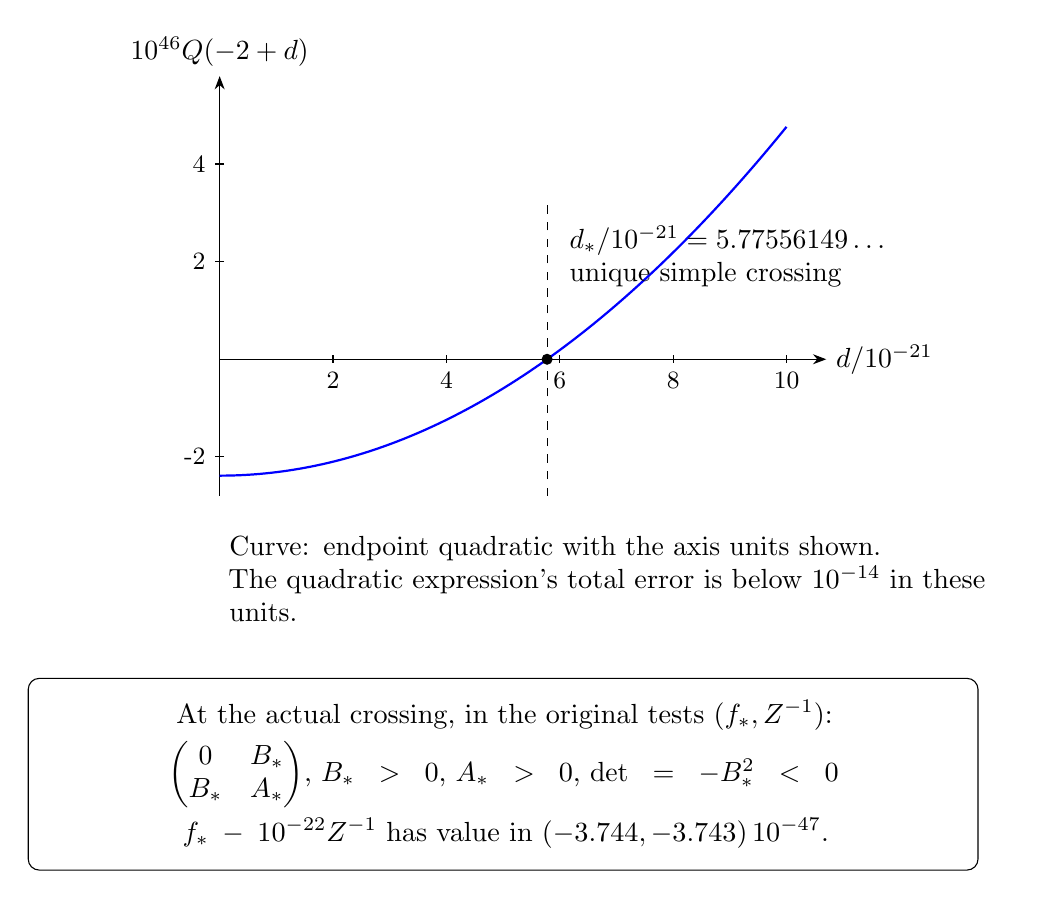
\begin{tikzpicture}[>=Stealth,x=0.72cm,y=0.62cm]
\draw[->] (0,-2.8)--(0,5.8) node[above] {$10^{46}Q(-2+d)$};
\draw[->] (0,0)--(10.7,0) node[right] {$d/10^{-21}$};
\foreach \x in {2,4,6,8,10}{\draw(\x,0.08)--(\x,-0.08) node[below] {\small\x};}
\foreach \y in {-2,2,4}{\draw(0.08,\y)--(-0.08,\y) node[left] {\small\y};}
\draw[thick,blue,domain=0:10,samples=100]
 plot(\x,{-2.384064178817915+0.07147094391701117*\x*\x});
\draw[dashed] (5.775561494,-2.8)--(5.775561494,3.2);
\fill (5.775561494,0) circle(2pt);
\node[anchor=west,align=left] at(6.0,2.1)
 {$d_*/10^{-21}=5.77556149\ldots$\\unique simple crossing};
\node[anchor=west,align=left,text width=10cm] at(0,-4.5)
 {Curve: endpoint quadratic with the axis units shown.\\
 The quadratic expression's total error is below $10^{-14}$ in these units.};
\node[draw,rounded corners,align=center,text width=11.5cm,inner sep=8pt]
 at(5,-8.5)
 {At the actual crossing, in the original tests $(f_*,Z^{-1})$:\\[3pt]
 $\begin{pmatrix}0&B_*\\B_*&A_*\end{pmatrix}$,
 $B_*>0$, $A_*>0$, $\det=-B_*^2<0$\\[3pt]
 $f_*-10^{-22}Z^{-1}$ has value in
 $(-3.744,-3.743)\,10^{-47}$.};
\end{tikzpicture}
\caption{The actual fixed-witness crossing and its surviving negative
direction. The axes record explicit display units only; time remains
$t=-2+d$ and the original test coefficients are unchanged. The curve
uses the endpoint quadratic (NC9--10); the displayed error bound also
includes its omitted linear term and coefficient rounding. NC12--14
give the rigorous crossing, and NC17--20 give the complete two-test
matrix and negative companion. The full theta source is Rodgers--Tao
(cited above); the vector is the supplied rational witness.}
\end{figure}

\end{document}
